%!TEX root=tese.tex
\chapter{Modelação e aplicação prática da separação pDNA/RNA por ultrafiltração}
\label{chap:art4}

\section{Introdução}
\label{sec:art4_intro}
Como referido no capítulo~\ref{chap:intro}, na última década tem sido efetuado um enorme esforço de investigação na área da recuperação e purificação de DNA plasmídico (pDNA) a partir de caldos de fermentação, com o objetivo de facilitar a sua produção em larga-escala, para aplicações em terapia génica e para a formulação de vacinas de DNA \cite{prather,carnes,meu2}. Os processos de separação com membranas estão presentes em praticamente todas as áreas da biotecnologia, numa grande variedade de aplicações \cite{rathore,reis}, e revelam o mesmo potencial de aplicação em processos de produção de DNA plasmídico \cite{carnes,prather,flowsheets}.

A recuperação e posterior purificação de pDNA a partir de caldos de fermentação, que pode ser efetuada por variadas técnicas, tipicamente envolve um passo de lise celular seguido por uma operação de separação sólido-líquido, subsequente precipitação de pDNA com álcoois tais como etanol ou isopropanol (ou mesmo outros agentes precipitantes), ressuspensão do concentrado de pDNA e sua posterior separação de RNA e outros contaminantes por técnicas de adsorção, que tipicamente são técnicas cromatográficas.
\index{caldos de fermentação}%
Estas técnicas cromatográficas são igualmente necessárias, num grande número de esquemas de purificação, para obter a isoforma super-enrolada do plasmídeo, pDNA(sc), com os requisitos de qualidade do produto final, impostos pelas entidades reguladoras, tais como a FDA (U.S.\ Food and Drug Administration) e a EMA (``European Medicines Agency'') \cite{prather,carnes,sousabab}.
\index{isoforma!super-enrolada}%
\index{EMA}%
\index{FDA}%

Operações de membranas foram utilizadas com sucesso para obter a colheita de células, a partir de caldos de fermentação, não só em processos de produção de pDNA como também em processos similares que envolvem suspensões celulares \cite{prather,riesmeier,morao01,brites} e igualmente para a seletiva retenção de detritos celulares, resultantes do processo de lise, permitindo a permeação de moléculas de pDNA \cite{duvaltff,meu3,freitas}. Estas operações foram já igualmente utilizadas na concentração de pDNA, com simultânea troca de tampão e remoção de micro-solutos, a seguir a operações de purificação cromatográfica, assim como para a esterilização do produto final \cite{prather,kong06,kong10}. Para além destas aplicações, as operações de membranas podem ser uma alternativa viável na fase da concentração e pré-purificação do pDNA antes da cromatografia, substituindo o uso de solventes e outros agentes precipitantes. 

A aplicação da ultrafiltração para efetuar a separação entre pDNA e RNA, assim como outros contaminantes, tem vindo a ser estudada por vários autores independentes. Kendall \et\ \cite{kendall} estudaram a purificação de pDNA através da adsorção seletiva de contaminantes em membranas de nitrocelulose.
\index{membrana!nitrocelulose}%
O procedimento desenvolvido permitiu remover quantidades significativas de RNA, DNA genómico e outros contaminantes hidrofóbicos.
\index{DNA genómico}%
No entanto, os problemas relacionados com a colmatação e a reduzida capacidade de membranas para atuarem como materiais adsorventes, podem ser sérias limitações da aplicação prática deste método. Eon-Duvall \et\ \cite{duvaltff} adicionaram cloreto de cálcio aos lisados e efetuaram uma subsequente operação de ultrafiltração para obter uma quase completa remoção de RNA.
\index{cloreto de cálcio!precipitação RNA}%
O facto de ser necessário utilizar uma elevada quantidade de \tce{CaCl2} é assim uma desvantagem do método. Kahn \et\ \cite{kahn} estudaram a aplicação da ultrafiltração de diferentes plasmídeos para obter a concentração de pDNA, e a sua separação do RNA, após um processo modificado de lise alcalina.
\index{lise alcalina!método modificado}%
Este método contempla um aumento do tempo de incubação (24 horas) durante a lise para obter uma degradação do RNA presente e assim obter elevados graus de purificação de pDNA com uma única operação de ultrafiltração. No entanto, o processo desenvolvido tem a desvantagem de conter elevados tempos de incubação para ser possível efetuar a separação, e não é claro que o pDNA não possa igualmente sofrer alguma degradação nestas condições. Freitas \et\ \cite{freitas} utilizaram um processo de ultrafiltração para efetuar uma recuperação intermediária de pDNA antes de um passo final de purificação. Apesar de obterem rendimentos de recuperação de pDNA elevados, o rendimento de remoção de RNA revelou-se ser modesto. 

Tendo em conta o estudo prévio, descrito no capítulo anterior, neste capítulo é investigada a possibilidade de otimizar a operação de ultrafiltração, procurando obter uma elevada retenção de pDNA e uma permeação alta dos principais contaminantes, com especial enfoque no RNA. A purificação de dois plasmídeos diferentes, \pVAX\ e \pCAMBIA, com 6050\,bp e 12361\,bp respetivamente, usando duas membranas de ultrafiltração distintas, é estudada numa célula de filtração agitada.
\index{pVAX@\pVAX}%
\index{pCAMBIA@\pCAMBIA}%
Os efeitos do tamanho do poro das membranas, da velocidade de agitação e do fluxo de filtração na separação entre pDNA e RNA, bem como no grau de colmatação das membranas, são interpretados com base no modelo desenvolvido para a permeação de macrosolutos flexíveis em membranas com poros de menores dimensões (capítulos~\ref{chap:art1}--\ref{chap:art3}). Para obter um termo comparativo, é avaliada a performance de um processo de isolamento intermediário alternativo, com base em duas operações de precipitação seletiva, usado com regularidade em laboratório e com o qual se obtêm resultados satisfatórios no âmbito do isolamento intermediário de pDNA \cite{sousabab,freitas}. 

\section{Materiais e métodos} % (fold)
\label{sec:art4_materias}
\subsection{Produção de pDNA e lise celular} % (fold)
\label{ssub:art4_lise}
Bactérias \emph{E. coli} DH5$\alpha$, contendo um plasmídeo de 6050\,bp (\pVAX), e bactérias \emph{E. coli} XL1\,blue, contendo um plasmídeo de 12361\,bp (\pCAMBIA) foram produzidas por fermentação, usando as mesmas condições de crescimento descritas em \cite{asousa}.
\index{ecolidh@\ecolidh}%
\index{ecolix@\emph{E. coli} XL1\,blue}%
\index{fermentação}%
As bactérias com o plasmídeo \pVAX\ foram cultivadas no meio Terrifc broth (12\,g/L de triptona (\emph{Sigma}), 24\,g/L de extrato de leveduras (\emph{Fluka}), 4\,mL/L de glicerol (\emph{Himedia}), 0.017\,M de \tce{KH2PO4} (\emph{Panreac}) e 0.072\,M de \tce{K2HPO4} (\emph{Panreac}), e as bactérias contendo o plasmídeo \pCAMBIA\ cultivadas em meio Luria Bertani (10\,g/L de triptona, 5\,g/L de extrato de leveduras, 10\,g/L de NaCl (\emph{Panreac}), pH 7.00).
\index{Terrific broth}%
\index{Luria Bertani}%
A lise celular foi obtida por um método modificado de lise alcalina, originalmente desenvolvido por Birnboim e Doly \cite{birnboim}.
\index{lise alcalina!procedimento}%
Resumidamente, a 4\,mL de uma suspensão de bactárias a 120\,g/L (peso húmido), em tampão $\mr{T}_{50}\mr{E}_{10}$ (50\,mM Tris (\emph{Fisher BioReagents}) e 10\,mM EDTA (\emph{Sigma}), pH 8.00), foram adicionados 4\,mL de uma solução de 0.2\,M de NaOH (\emph{Panreac}) e 1\% SDS (\emph{Himedia}). Após 5\,min de incubação a temperatura ambiente, foram adicionados 4\,mL de uma solução previamente arrefecida (4\degreecelsius) de 3\,M de acetato de potássio (\emph{Sigma-Aldrich}) a pH 5.00, com o pH ajustado com ácido acético (\emph{Panreac}). Após agitação suave, a suspensão obtida foi incubada em gelo durante 15\,min antes de ser processada por microfiltração.  
% subsubsection art4_lise (end)

\subsection{Clarificação de lisados - Microfiltração} % (fold)
\label{ssub:2.2art4}
\index{lisado!clarificação}%
O lisado alcalino obtido, contendo uma grande quantidade de sólidos em suspensão, foi filtrado por microfiltração usando uma membrana hidrofílica de Nylon (Nylaflo, \emph{Pall}), com um tamanho de poro nominal de 0.2\,\micro\meter.
\index{Nylon}%
\index{Nylaflo|see{Nylon}}%
Foi efetuada uma diafiltração continua numa célula de filtração agitada, com geometria ``dead-end'', com 50\,mL de capacidade (modelo 8050, \emph{Millipore}).
\index{Amicon 8050}%
A velocidade de agitação foi mantida a 100\,\minmum\ e o caudal de permeado ajustado, e mantido, em 1\,mL/min através de uma bomba peristáltica (modelo 403U/VM2, \emph{Watson Marlow}) colocada a jusante da membrana, operando assim por sucção.
\index{caudal volumétrico}%
\index{velocidade de agitação}%
\index{bomba peristáltica}%
O volume de lisado processado em cada ensaio foi de 10\,mL. O volume da suspensão no interior da célula de filtração foi mantido constante através da contínua adição de Tris/HCl 10\,mM a pH 8.00 (tampão Tris), que foi alimentado à célula de filtração através de uma segunda bomba peristáltica (modelo 101U/R, \emph{Watson Marlow}), ao mesmo caudal.
\index{Tris}%
A filtração foi concluída após a recolha de um total de 30\,mL de permeado. Nestas condições espera-se um rendimento de recuperação de plasmídeo no permeado de cerca de 95\%, considerando que o plasmídeo não é retido pela membrana, fazendo uso da equação do balanço de massa para o modo de diafiltração a volume constante (equação~\ref{bal_mas_df_final}, capítulo~\ref{cha:pra}).
\index{DNA plasmídico!rendimento de recuperação}%
\index{rendimento!de recuperação}%
% subsubsection 2.2art4 (end)

\subsection{Ultrafiltração} % (fold)
\label{ssub:2.3art4}
\index{ultrafiltração}%
Os ensaios de ultrafiltração foram efetuados numa célula de filtração Amicon 8010, com geometria ``dead-end'' (\emph{Millipore}).
\index{Amicon 8010}%
Em todos os ensaios, o volume inicial de lisado alcalino microfiltrado foi de 10\,mL, tendo-se recolhido 9\,mL de permeado, o que equivale a um fator de concentração volumétrico (VCF) igual a 10.
\index{fator!de concentração}%
Testaram-se duas membranas distintas: uma membrana de 100\,kDa de ``cut-off'' de polímero fluorado (FS40PP, \emph{DSS/Alfa-laval}) e uma membrana de 300\,kDa de ``cut-off'' de polietersulfona (Biomax\,300, \emph{Millipore}).
\index{FS40PP}%
\index{Biomax 300}%
\index{PVDF}%
\index{polietersulfona}%
Estas membranas foram previamente caracterizadas, em relação ao tamanho de poro, através do modelo de poros simétricos (SPM) desenvolvido por Morão \et\ \cite{moraompa}.
\index{modelo!dos poros simétricos}%
O caudal de permeado foi mantido constante através do uso de uma bomba peristáltica (modelo 101U/R, \emph{Watson Marlow}), colocada a jusante da membrana. A velocidade de agitação foi ajustada a 100 ou a 760\,\minmum, com calibração prévia.
\index{caudal de permeado}%   
% subsubsection 2.3art4 (end)

\subsection{Isolamento intermediário usando tecnologias de membranas} % (fold)
\label{sub:isol_mem_final}
\index{isolamento intermediário}%
Foram efetuados três conjuntos de ensaios, para o isolamento intermediário de pDNA, com o objetivo de melhorar os valores de remoção de RNA, recorrendo a uma operação de diafiltração. Os ensaios foram todos efetuados em triplicado, tendo-se obtido uma boa reprodutibilidade entre os mesmos. O esquema dos ensaios efetuados, bem como as principais condições operatórias utilizadas, estão representados na figura~\ref{fig:processos_art4} e tabela~\ref{tab:cond_isolamento_art4}, respetivamente. As experiências foram conduzidas numa célula de filtração agitada, com 10 mL de capacidade, com geometria ``dead-end'' (Amicon 8010, \emph{Millipore}). A agitação foi mantida a 760\,\minmum\ em todos os ensaios. O caudal de permeado foi imposto através de uma bomba peristáltica (WM101U/R, \emph{Watson Marlow}). Foram usadas novamente as membranas FS40PP e Biomax\,300. Antes de se iniciar a filtração, as membranas foram lavadas com a filtração de pelo menos 30\,mL de água MilliQ (\emph{Millipore}). Após lavagem das membranas, as suas permeabilidades hidráulicas foram medidas através da determinação do fluxo de água em função da pressão transmembranar, pressão esta imposta pela ligação da célula de filtração a uma garrafa de azoto pressurizado. Foram colocados inicialmente na célula 10 mL de permeado proveniente da microfiltração do lisado. O permeado foi concentrado a um fator de concentração volumétrico (VCF) predefinido (ver tabela~\ref{tab:cond_isolamento_art4}), segundo o método descrito na secção~\ref{ssub:2.3art4}. Após concluída a concentração, foi efetuada uma diafiltração com aproximadamente 4 volumes de diafiltração ($V_{\mr{DF}}$) de Tris/HCl 10 mM a pH 8.00 (tampão Tris), ao mesmo caudal, e utilizando uma segunda bomba peristáltica (WM403U/R, \emph{Watson Marlow}).
\index{diafiltração}%
Foram recolhidas amostras da solução inicial antes da concentração (permeado da microfiltração), do concentrado após diafiltração e do permeado conjunto da fase de concentração e da fase de diafiltração, para posterior análise. Para aferir o grau de colmatação irreversível das membranas usadas, no fim dos ensaios a célula foi lavada com água MilliQ, com agitação suave e breve, e a permeabilidade hidráulica novamente determinada.
% subsection isol_mem_final (end)

\begin{figure}
\centering
	\begin{tikzpicture}

\node[anchor = south west] at (0cm, 0cm) {%\includegraphics[width=7cm]{% mudar para 6.3 cm
\includegraphics[width=14cm]{processos_art4.jpg}};

% \draw[help lines] (0cm, -2cm) grid (14cm, 10cm);

\node[align = center] at (1.5, 4.5) {Filtração lisado \\ (Microfiltração)};
\node[align = center] at (4.5, 4.5) {Concentração \\ (Ultrafiltração)};
\node[align = center] at (7.4, 4.5) {Diafiltração \\ (Ultrafiltração)};

\node[align = center] at (1.5, -0.5) {Centrifugação \\ lisado};
\node[align = center] at (4.4, -0.5) {Precipitação \\ isopropanol};
\node[align = center] at (7.4, -0.5) {Centrifugação \\ \phantom{phantom}};
\node[align = center] at (10.3, -0.5) {Precipitação \\ sulfato de amónio};
\node[align = center] at (13.3, -0.5) {Centrifugação \\ \phantom{phantom}};

\draw[dashed] (3, 4) rectangle (8.9, 7.4);
\draw[dashed] (3, -1) rectangle (14.5, 3.5);

\node[right, align = left] at (9, 6.7) {Processo A:\\FS40PP (\pVAX)};
\node[right, align = left] at (9, 5.7) {Processo B:\\Biomax\,300 (\pVAX)};
\node[right, align = left] at (9, 4.7) {Processo C:\\Biomax\,300 (\pCAMBIA)};
\node at (9.25, -1.5) {Processo D: processo alternativo};

\end{tikzpicture}
	\caption[Esquemas dos processos de isolamento intermediário estudados]{Esquema dos processos estudados de isolamento intermediário de pDNA. A tracejado encontram-se as operações consideradas nos cálculos. Os processos A--C usam exclusivamente operações de membranas. O processo D consiste no procedimento de isolamento intermediário alternativo, descrito em \cite{sousabab}. As condições operatórias para os processos A--C estão especificadas na tabela~\ref{tab:cond_isolamento_art4}.}
	\label{fig:processos_art4}  
\end{figure}
%
\begin{table}[!b]
	\caption[Condições operatórias utilizadas nos ensaios de isolamento intermediário.]{Condições operatórias, utilizadas nos processos com base em tecnologias de membrana, para efetuar o isolamento intermediário de pDNA.}
	\label{tab:cond_isolamento_art4}
\begin{tabular*}{\textwidth}{l@{\extracolsep{\fill}}l l d{9} d{5} d{2} d{6}}
 \toprule
Processo & Membrana & pDNA & \mc{1}{l}{\fluxo$\times 10^{6}$\,[m/s]} & \mc{1}{l}{\agitacao\,[\minmum]} & \mc{1}{l}{VCF} & \mc{1}{l}{$V_{\mr{DF}}$\,[mL]} \\
\midrule
``A'' & FS40PP & \pVAX & 4,2 & 760 & 8 & 3,8 \\
``B'' & Biomax\,300 & \pVAX & 2,4 & 760 & 8,4 & 4 \\
``C'' & Biomax\,300 & \pCAMBIA & 2,4 & 760 & 8,4 & 4 \\
\bottomrule
\end{tabular*}
\end{table}

\subsection{Isolamento intermediário alternativo} % (fold)
\label{sub:isol_alter_final}
\index{isolamento intermediário alternativo}%
Para se obter um termo comparativo, em relação aos resultados obtidos com os ensaios de ultrafiltração/diafiltração, foi igualmente estudado um processo de isolamento intermediário alternativo (Processo D, figura~\ref{fig:processos_art4}), regularmente usado em laboratório \cite{sousabab,freitas}. Foi efetuado o procedimento descrito em \cite{sousabab}. O lisado, proveniente da lise alcalina, foi centrifugado duas vezes a 19\,000\,g, durante 30\,min e a 4\degreecelsius, numa centrífuga Allegra 25R (\emph{Beckman Coulter}).
\index{centrifugação}%
Ao sobrenadante obtido (8\,mL) foram adicionados 0.7 volumes de isopropanol (\emph{Fischer}).
\index{isopropanol!isolamento intermediário alternativo}%
Após 30\,min de incubação em gelo, a suspensão foi centrifugada durante 30\,min, a 16\,000\,g e 4\degreecelsius, na mesma centrífuga. Após remoção do sobrenadante, o ``pellet'' foi dissolvido em 2.5\,mL de tampão Tris. Foi adicionado sulfato de amónio (\emph{Prolabo, VWR}) até perfazer uma concentração de 2.5\,M.
\index{sulfato de amónio!isolamento intermediário alternativo}%
Após incubação durante 15 min em gelo, a suspensão foi centrifugada a 16\,000\,g, durante 20\,min e 4\degreecelsius, numa centrífuga Mikro 200R (\emph{Hettich}). Foram recolhidas amostras ao longo do processo para posterior análise.

\subsection{Parte analítica} % (fold)
\label{ssub:2.4art4}
\subsubsection{Quantificação de pDNA e RNA}
\label{ssubsub:2.4.1art4}
\index{HIC}%
\index{plasmídeo|see{DNA plasmídico}}%
A concentração de plasmídeo nas várias amostras foi determinada pelo método desenvolvido por Diogo \et\ \cite{diogo}. Resumidamente, uma coluna HIC \emph{source 15} PHE, da \emph{Amersham Biosciences (GE Healthcare)} foi conectada a um sistema de FPLC (\emph{Äkta purifier}) da \emph{GE Healthcare}.
\index{akta@Äkta}%
A coluna foi inicialmente equilibrada com 1.5\,M de \tce{(NH4)2SO4} em tampão tris. As amostras (20\,\micro L) foram injetadas e eluídas a um caudal constante de 1\,mL/min. Ao fim de 2\,min após a injeção, o eluente foi instantaneamente mudado para tampão Tris para eluir as espécies adsorvidas. Este tampão foi mantido por mais 4\,min antes de se re-equilibrar a coluna para a preparar para a próxima injeção. A absorvância do eluído foi registada a 260\,nm. A concentração de pDNA em cada amostra foi calculada por intermédio de uma reta de calibração, preparada com padrões de pDNA obtidos com um kit de purificação (\emph{Maxi kit, Qiagen}). Este método está descrito em detalhe no capítulo~\ref{cha:pra}, onde se propõe que a concentração de RNA pode igualmente ser estimada.    
% subsubsection 2.4art4 (end)

\subsubsection{Eletroforese em gel de agarose} % (fold)
\label{ssub:2p4p1art4}
\index{AGE!procedimento}%
As amostras foram analisadas por eletroforese horizontal, em gel de 1.0\% de agarose (\emph{Grisp}), preparado em tampão TAE (40\,mM Tris, 20\,mM ácido acético e 1\,mM de EDTA, pH 8.00), complementado com o corante \emph{GreenSafe} (\emph{NZYTech}).
\index{greensafe@\emph{GreenSafe}}%
As análises decorreram a 110\,V, durante 40\,min, numa célula da \emph{BioRad}. Os géis foram visualizados num transiluminador da \emph{Uvitec}, modelo \emph{Essential V2}.
\index{transiluminador}%
Para concentrar, e/ou evitar possíveis interferências provocadas pelos sais presentes, algumas amostras foram dessalinizadas, através de precipitação com isopropanol, tal como descrito no capítulo~\ref{chap:art3}.
\index{isopropanol!dessalinização}%
% subsubsection 2p4p1art4 (end)

\subsection{Simulações} % (fold)
\label{sub:2p5art4}
Para efetuar uma otimização da operação de ultrafiltração, com o intuito de obter uma elevada retenção de pDNA e uma elevada permeação de RNA, efetuaram-se simulações, quer para um sistema de 3 componentes contendo a macromolécula de interesse (pDNA ou RNA, componente 1), ião acetato (componente 2) e ião potássio (componente 3), quer para um sistema de 4 componentes contendo o plasmídeo, uma espécie de RNA (23S, 16S ou 5S), o ião acetato e o ião potássio.
\index{modelo!3 componentes}%
\index{modelo!4 componentes}%
Nas simulações utilizou-se o método descrito nos capítulos~\ref{chap:teov3}, \ref{chap:art2} e \ref{chap:art3}. Apesar de nos lisados microfiltrados existirem outros sais presentes em solução, os iões \tce{CH3COO-} e \tce{K+} são, por larga margem, os que se encontram em maior quantidade, sendo os principais responsáveis pelos efeitos de carga que afetam em grande medida a polarização de concentração de macrosolutos (pDNA e RNA) que são altamente carregados negativamente.
\index{iao@ião!potássio}%
\index{iao@ião!acetato}%

O modelo de transferência de massa anteriormente desenvolvido permite estimar a permeação de macrosolutos em membranas com poros de reduzidas dimensões, ou seja, poros com um raio médio inferior ao raio de giração do macrosoluto, sendo que este último deverá apresentar alguma flexibilidade. Este modelo foi originalmente desenvolvido para moléculas lineares, que foram modeladas como cadeias de ligação livre (FJC), nomeadamente para pDNA linear e para polissacáridos lineares (capítulo~\ref{chap:art1}). O modelo foi estendido ao caso de macrosolutos de cadeia fechada, através da sua representação pelo modelo de cadeias fechadas segmentadas (CSC), discutido nos capítulos~\ref{chap:teov3}~e~\ref{chap:art2}. De facto, verificou-se que a equação obtida, que relaciona o rácio entre o raio de giração da molécula e o raio do poro com o coeficiente de partição, pode ser usada quer para cadeias FJC quer para cadeias CSC (capítulo~\ref{chap:art2}). Apesar de uma molécula de pDNA poder ser modelada como uma FJC, a representação CSC é, aparentemente, uma melhor aproximação por permitir obter valores de raio de giração em melhor concordância com os valores encontrados na literatura. O modelo desenvolvido pode igualmente ser usado para prever a permeação de RNA, considerando-o uma molécula linear, ou seja, utilizando o modelo FJC, tal como indicado no capítulo~\ref{chap:art3}, onde se aplicou o modelo de 3 componentes para prever a permeação das principais espécies de RNA presentes nos lisados, nomeadamente os RNA's 23S, 16S e 5S, de forma individual. 

Neste capítulo investiga-se a possível mútua interferência entre pDNA e RNA nas suas permeações, considerando um sistema de 4 componentes. A inclusão de um maior número de componentes no modelo representa uma interpretação mais realista do fenómeno mas aumenta consideravelmente a complexidade dos cálculos e o esforço computacional necessário. Para além disso, tal como mostrado mais à frente, a principal interferência é o efeito do pDNA na permeação do RNA e não o contrário, sendo que este último efeito pode ser simulado com um sistema de 4 componentes. 

As simulações do processo de ultrafiltração foram levadas a cabo considerando um cenário de filtração numa célula agitada, com 10\,mL de solução inicial (permeado da microfiltração), em condições de fluxo e velocidade de agitação constantes e em modo de concentração, cenário este consistente com o procedimento experimental descrito na secção~\ref{ssub:2.3art4}. As concentrações inicias das macromoléculas e sais usados nas simulações, assim como as suas propriedades mais relevantes, estão indicadas na tabela~\ref{tab:1art4}. As várias propriedades das moléculas foram determinadas pelos métodos discutidos na secção~\ref{sec:solutos}. 
\begin{table}
	\caption[Componentes e suas propriedades relevantes]{Principais componentes do lisado microfiltrado e as suas propriedades mais relevantes para fins de modelação.}
	\label{tab:1art4}
\begin{threeparttable}
\begin{tabular*}{15cm}{l@{\extracolsep{\fill}} l d{0} d{6} d{6} d{8} }
\toprule
Componente\phantom{MM}&\concb\,[mol/$\mr{m}^3$]&\mc{1}{r}{M$\mr{_w}$\,[Da]\phantom{l}}&\mc{1}{l}{$\raiostokes\times 10^9$\,[m]}&\mc{1}{l}{$\raiogiracao\times 10^9$\,[m]} & \mc{1}{l}{$D\times 10^{12}\,[\mr{m}^2/\mr{s}]$}\\
\midrule
\tce{CH3COO-} & $3.17\times 10^2$ & 59 & 0,227 &  & 1089\\
\tce{K+}	     & $3.17\times 10^2$ & 39 & 0,125 &  & 1950 \\
RNA 5S              & $2.26\times 10^{-3}$\tnote{a} & 40800 & 3,39 & 5,10 & 72,9\tnote{c}\\
                          & $8.45\times 10^{-4}$\tnote{b} &            &         &          &            \\
RNA 16S            & $1.06\times 10^{-4}$\tnote{a} & 523940 & 13,6 & 20,5 & 18,2\tnote{c}\\ 
                          & $8.99\times 10^{-5}$\tnote{b} &              &          &         &           \\
RNA 23S            & $5.63\times 10^{-5}$\tnote{a} & 987360& 17,8 & 26,8 &  13,9\tnote{c} \\
                          & $4.77\times 10^{-5}$\tnote{b} &             &         &         &           \\
\pVAX                 & $4.47\times 10^{-6}$\tnote{a} & 3993000 & 83,1 & 87,3 & 2,97\tnote{d}\\
\pCAMBIA                          & $6.39\times 10^{-7}$\tnote{b} & 8158260 & 134 & 138,7 & 1,85 \tnote{d}\\
\bottomrule
\end{tabular*}
\begin{tablenotes}
\item[a] Lisados provenientes da produção de \pVAX  
\item[b] Lisados provenientes da produção de \pCAMBIA
\item[c] Valores obtidos no capítulo~\ref{chap:art3}
\item[d] Valores obtidos em \cite{prazeresdif}
\end{tablenotes}
\end{threeparttable}
\end{table}
% subsection 2p5art4 (end)
% section art4_materias (end)

\section{Resultados e discussão} % (fold)
\label{sec:3art4}
\subsection{Simulações} % (fold)
\label{sub:3.1art4}
Para proceder à otimização de uma operação de ultrafiltração, com o objetivo de concentrar o pDNA e simultâneamente proceder à sua separação do RNA presente, o raio do poro da membrana, \raioporo, e o fluxo de filtração, \fluxo, devem ser os primeiros parâmetros a considerar. Em seguida, deve-se testar o material da membrana, nomeadamente em termos da sua suscetibilidade à colmatação e adsorção de plasmídeo, que deve ser o mais reduzida possível. Assim, os efeitos de \raioporo\ e \fluxo\ nas permeações das moléculas indicadas na tabela~\ref{tab:1art4} foram estimados antes dos ensaios experimentais. As previsões foram efetuadas considerando quer o modelo de 3 componentes, quer o modelo de 4 componentes, descritos na secção~\ref{sub:2p5art4}, em condições ideais de ausência de colmatação e adsorção de pDNA e RNA.

O efeito previsto das diferentes moléculas de RNA na permeação observada, \permobs, do plasmídeo \pVAX, calculada pelos dois modelos propostos, é analisado na figura~\ref{fig:1abcart4}. Obtiveram-se resultados semelhantes para o plasmídeo \pCAMBIA\ (resultados não mostrados).
\index{pVAX@\pVAX!permeação observada}%
\index{pCAMBIA@\pCAMBIA!permeação observada}%
Como é possível constatar, observa-se apenas um ligeiro decréscimo de \permobs, o que leva a concluir que este efeito pode ser desprezado (pelo menos para as concentrações consideradas nos cálculos). Apesar da presença das moléculas de RNA não interferirem significativamente na permeação de pDNA, a presença de pDNA influencia consideravelmente a permeação das moléculas de RNA. Como se pode observar na figura~\ref{fig:2art4}, um significativo decréscimo de \permobs\ é previsto, especialmente a altos valores de fluxo e para as espécies de RNA de alto peso molecular (ou seja, RNA 23S e 16S).
\index{RNA!permeação observada}%
Os resultados das simulações podem ser interpretados considerando a polarização de concentração esperada para cada componente, expressa pelo rácio $\concm/\concb$, onde \concm\ é a concentração junto à superfície da membrana e \concb\ é a concentração no seio da solução. Os valores calculados de $\concm/\concb$ para o plasmídeo \pVAX, e para as várias espécies de RNA, estão indicados nas figuras~\ref{fig:3aart4}~e~\ref{fig:3bcdart4}, respetivamente, para o caso de $\raioporo=5$\,nm (para $\raioporo=15$\,nm e $\raioporo=25$\,nm podem ser obtidas conclusões semelhantes). Como é possível constatar na figura, existe uma maior acumulação de moléculas de pDNA junto à membrana, por comparação com as moléculas de RNA, o que é consequência dos menores coeficientes de difusão das moléculas de pDNA. Esta acumulação de pDNA afeta a acumulação de RNA (e provavelmente de outras moléculas carregadas negativamente presentes em solução, que não foram consideradas neste estudo) reduzindo a polarização de concentração por efeitos de repulsão eletrostática.
\index{repulsão!eletrostática}%
Como é sabido, o decréscimo de polarização de concentração de um componente reduz a sua permeação observada. O efeito da presença de moléculas de RNA na polarização de concentração de pDNA é claramente menos significativo, o que se deve ao facto das moléculas de RNA apresentarem um tamanho inferior e serem menos carregadas negativamente (assim, só para concentrações altas de RNA são esperados efeitos significativos).
\begin{figure}
	\centering
	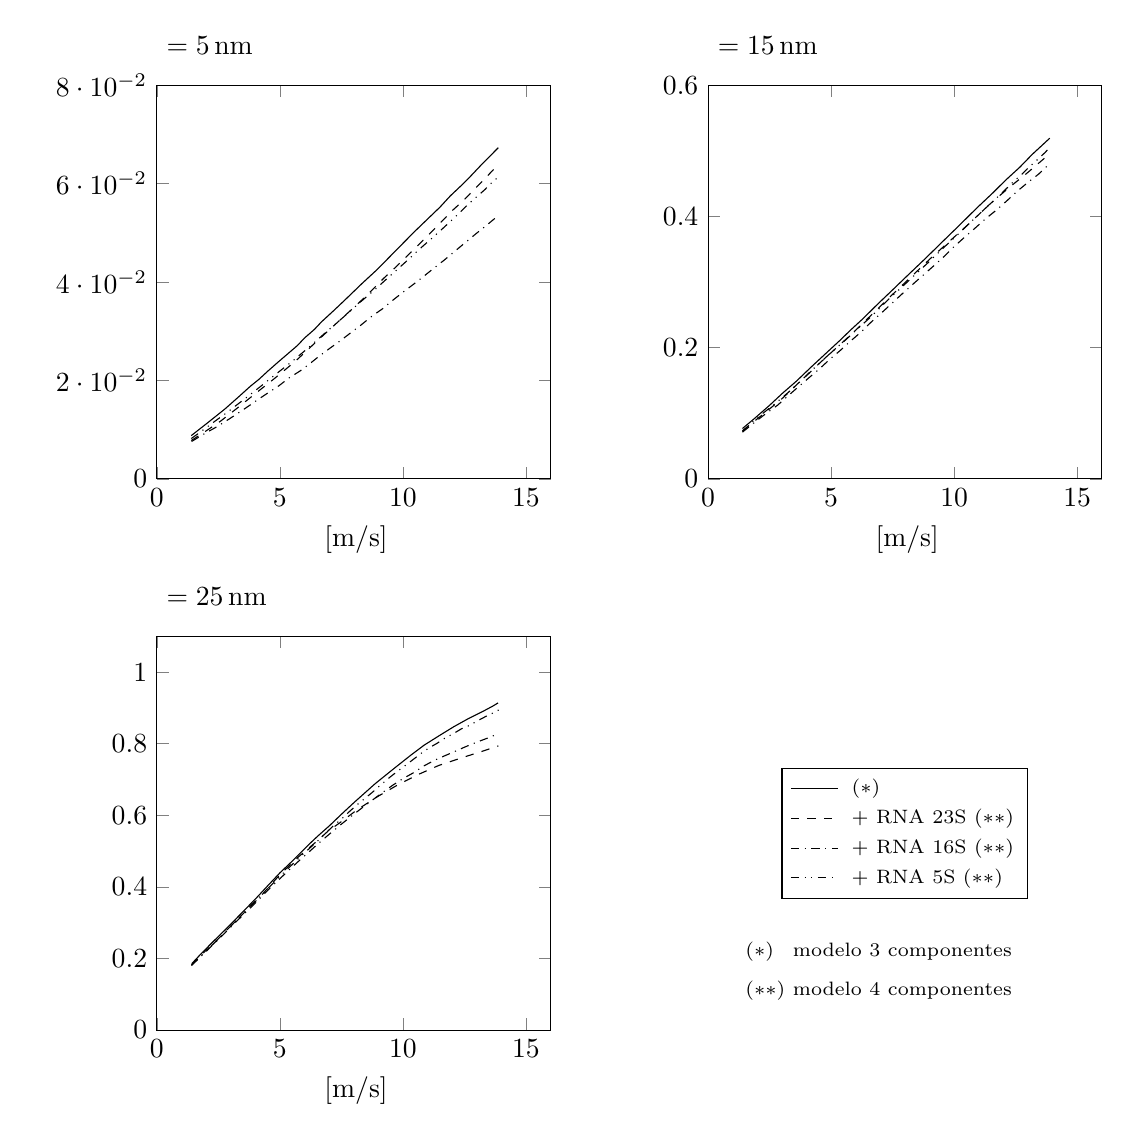
\begin{tikzpicture}

%\node[below right] at (0cm,12cm) {$\raioporo=5$\,nm};
%\node[below right] at (7cm,12cm) {$\raioporo=15$\,nm};
%\node[below right] at (0cm,5cm) {$\raioporo=25$\,nm};

\node[right] at (0cm,12.5cm) {$\raioporo=5$\,nm};
\node[right] at (7cm,12.5cm) {$\raioporo=15$\,nm};
\node[right] at (0cm,5.5cm) {$\raioporo=25$\,nm};

\node[right,font=\scriptsize] at (7.35cm,1cm) {($\ast$)\phantom{$\ast$} modelo 3 componentes}; 
\node[right,font=\scriptsize] at (7.35cm,0.5cm) {($\ast\ast$) modelo 4 componentes};

%\node[left,font=\scriptsize] at (7cm,1cm) {$\ast$};
%\node[left,font=\scriptsize] at (7cm,0.5cm) {$\ast\ast$};

\begin{axis}[%
scaled ticks=false,
width=5cm,
height=5cm,
forget plot,
scale only axis,
xmin=0,
xmax=16,
xlabel={\fluxo\,[\micro m/s]},
ymin=0,
ymax=0.08,
ylabel={\permobs},
at={(0cm,7cm)},
anchor=south west
]

\addplot[
color=black,
solid
]
table[row sep=crcr]{
1.3984 0.0088\\
2.0379 0.0113\\
2.7642 0.0142\\
3.3062 0.0166\\
3.7940 0.0188\\
4.1409 0.0202\\
4.5095 0.0219\\
4.9648 0.0239\\
5.7127 0.0271\\
5.9946 0.0286\\
6.4065 0.0304\\
6.6883 0.0319\\
7.2087 0.0343\\
7.6314 0.0363\\
8.3360 0.0397\\
8.9648 0.0426\\
9.6911 0.0463\\
10.461 0.0502\\
10.959 0.0526\\
11.501 0.0552\\
11.924 0.0575\\
12.390 0.0597\\
12.748 0.0615\\
13.182 0.0638\\
13.875 0.0673\\
};
\addplot[
color=black,
dashed
]
table[row sep=crcr]{
1.3984 0.0078\\
1.8645 0.0093\\
2.5799 0.0117\\
3.2954 0.0145\\
3.9675 0.0172\\
4.7046 0.0201\\
5.1924 0.0221\\
5.6043 0.0238\\
5.9946 0.0256\\
6.5474 0.0282\\
7.4038 0.0321\\
8.1734 0.0356\\
8.7913 0.0386\\
9.2249 0.0408\\
9.6585 0.0428\\
10.049 0.0447\\
10.417 0.0465\\
10.862 0.0487\\
11.241 0.0506\\
11.653 0.0527\\
12.000 0.0545\\
12.466 0.0566\\
12.835 0.0585\\
13.312 0.0609\\
13.648 0.0627\\
13.897 0.0639\\
};
\addplot[
color=black,
dashdotted
]
table[row sep=crcr]{
1.4092 0.0076\\
1.9404 0.0092\\
2.4390 0.0106\\
2.9160 0.0121\\
3.2846 0.0133\\
3.7290 0.0148\\
4.1301 0.0162\\
4.5528 0.0176\\
4.9539 0.0189\\
5.3659 0.0205\\
5.8103 0.0219\\
6.2114 0.0234\\
6.6125 0.0250\\
7.0461 0.0266\\
7.4905 0.0282\\
7.8808 0.0297\\
8.3035 0.0313\\
8.7480 0.0331\\
9.1816 0.0346\\
9.5610 0.0362\\
9.9946 0.0379\\
10.417 0.0395\\
10.829 0.0411\\
11.252 0.0428\\
11.664 0.0444\\
12.119 0.0463\\
12.553 0.0481\\
12.965 0.0498\\
13.366 0.0514\\
13.897 0.0536\\
};
\addplot[
color=black,
dashdotdotted
]
table[row sep=crcr]{
1.3984 0.0082\\
1.7344 0.0094\\
2.2439 0.0113\\
2.9051 0.0137\\
3.5772 0.0163\\
4.2168 0.0188\\
4.8672 0.0214\\
5.5285 0.0240\\
6.1680 0.0267\\
6.8943 0.0299\\
7.5881 0.0329\\
8.2602 0.0359\\
8.8238 0.0383\\
9.4417 0.0411\\
10.070 0.0439\\
10.743 0.0470\\
11.404 0.0499\\
12.076 0.0530\\
12.694 0.0560\\
13.333 0.0588\\
13.669 0.0605\\
13.897 0.0614\\
};
\end{axis}

\begin{axis}[%
width=5cm,
height=5cm,
forget plot,
scale only axis,
xmin=0,
xmax=16,
xlabel={\fluxo\,[\micro m/s]},
ymin=0,
ymax=0.6,
ylabel={\permobs},
at={(7cm,7cm)},
anchor=south west
]
\addplot[
color=black,
solid
]
table[row sep=crcr]{
1.3984 0.0768\\
1.8537 0.0910\\
2.4932 0.1119\\
3.0244 0.1305\\
3.5989 0.1492\\
4.1626 0.1695\\
4.7805 0.1910\\
5.3659 0.2113\\
5.7995 0.2271\\
6.3089 0.2446\\
6.7642 0.2616\\
7.0894 0.2734\\
7.5014 0.2881\\
8.0325 0.3073\\
8.8238 0.3356\\
9.5610 0.3627\\
10.211 0.3864\\
10.927 0.4130\\
11.566 0.4356\\
12.098 0.4554\\
12.672 0.4751\\
13.171 0.4944\\
13.886 0.5192\\
};
\addplot[
color=black,
dashed
]
table[row sep=crcr]{
1.3984 0.0734\\
2.3415 0.1017\\
3.0678 0.1243\\
3.5989 0.1435\\
4.1518 0.1627\\
4.5312 0.1763\\
4.9431 0.1904\\
5.6260 0.2136\\
6.0921 0.2299\\
6.4932 0.2446\\
6.8726 0.2582\\
7.3930 0.2774\\
9.0298 0.3356\\
9.8103 0.3621\\
10.634 0.3898\\
11.415 0.4175\\
12.217 0.4435\\
12.932 0.4650\\
13.301 0.4768\\
13.691 0.4893\\
13.886 0.4949\\
};
\addplot[
color=black,
dashdotted
]
table[row sep=crcr]{
1.3984 0.0712\\
1.9187 0.0870\\
2.4065 0.1011\\
2.8293 0.1124\\
3.2520 0.1266\\
3.6640 0.1401\\
4.0867 0.1537\\
4.5312 0.1678\\
4.9539 0.1825\\
5.3659 0.1955\\
5.7778 0.2096\\
6.2005 0.2232\\
6.6125 0.2384\\
7.0352 0.2525\\
7.4797 0.2678\\
7.9024 0.2825\\
8.3035 0.2960\\
8.7480 0.3107\\
9.1599 0.3243\\
9.5935 0.3390\\
10.005 0.3542\\
10.428 0.3684\\
10.862 0.3825\\
11.263 0.3960\\
11.696 0.4090\\
12.141 0.4237\\
12.564 0.4384\\
12.965 0.4508\\
13.431 0.4644\\
13.897 0.4808\\
};
\addplot[
color=black,
dashdotdotted
]
table[row sep=crcr]{
1.3984 0.0723\\
1.9187 0.0910\\
2.5799 0.1102\\
3.2412 0.1311\\
3.7290 0.1480\\
4.2818 0.1678\\
4.9539 0.1910\\
5.6260 0.2130\\
6.0921 0.2294\\
6.5149 0.2435\\
6.9702 0.2599\\
7.3930 0.2757\\
7.8049 0.2898\\
8.4661 0.3130\\
8.9214 0.3288\\
9.5285 0.3508\\
10.114 0.3712\\
10.818 0.3966\\
11.566 0.4226\\
12.033 0.4390\\
12.369 0.4514\\
12.759 0.4644\\
13.030 0.4746\\
13.366 0.4859\\
13.691 0.4972\\
13.886 0.5051\\
};
\end{axis}

\begin{axis}[%
width=5cm,
height=5cm,
scale only axis,
xmin=0,
xmax=16,
xlabel={\fluxo\,[\micro m/s]},
ymin=0,
ymax=1.1,
ylabel={\permobs},
at={(0cm,0cm)},
anchor=south west,
legend style={at={(9.5cm,2.5cm)},legend columns=1,anchor=center,font=\scriptsize,draw=black,fill=white,legend cell align=left}
]
\addplot[
color=black,
solid
]
table[row sep=crcr]{
1.4181 0.1855\\
1.7429 0.2093\\
2.2625 0.2456\\
2.7713 0.2798\\
3.4533 0.3275\\
4.0271 0.3679\\
4.5034 0.4031\\
5.0014 0.4394\\
5.4777 0.4705\\
6.1705 0.5181\\
6.5386 0.5420\\
7.0149 0.5710\\
7.5020 0.6031\\
8.0217 0.6363\\
8.8660 0.6881\\
9.6130 0.7295\\
10.317 0.7679\\
10.858 0.7959\\
11.529 0.8249\\
12.070 0.8477\\
12.666 0.8705\\
13.272 0.8912\\
13.640 0.9047\\
13.867 0.9140\\
};\addlegendentry{\pVAX\ ($\ast$)}
\addplot[
color=black,
dashed
]
table[row sep=crcr]{
1.4073 0.1824\\
1.7645 0.2073\\
2.5115 0.2560\\
3.0419 0.2933\\
3.5399 0.3275\\
4.1894 0.3720\\
5.0122 0.4352\\
5.7375 0.4829\\
6.4628 0.5254\\
6.9499 0.5554\\
7.4587 0.5803\\
8.1624 0.6166\\
9.0068 0.6539\\
9.8403 0.6870\\
10.652 0.7150\\
11.442 0.7389\\
12.287 0.7585\\
13.099 0.7762\\
13.878 0.7938\\
};\addlegendentry{\pVAX\ + RNA 23S ($\ast\ast$)}
\addplot[
color=black,
dashdotted
]
table[row sep=crcr]{
1.4073 0.1803\\
2.0352 0.2218\\
2.8579 0.2777\\
3.2801 0.3067\\
3.7673 0.3389\\
4.1245 0.3637\\
4.5359 0.3927\\
4.9364 0.4187\\
5.3586 0.4466\\
5.7700 0.4725\\
6.1922 0.4984\\
6.6143 0.5244\\
7.0582 0.5503\\
7.4587 0.5731\\
7.8701 0.5959\\
8.3572 0.6218\\
9.1800 0.6642\\
9.5805 0.6839\\
10.003 0.7026\\
10.436 0.7192\\
10.847 0.7378\\
11.269 0.7534\\
11.713 0.7668\\
12.135 0.7793\\
12.547 0.7917\\
12.991 0.8041\\
13.391 0.8145\\
13.878 0.8280\\
};\addlegendentry{\pVAX\ + RNA 16S ($\ast\ast$)}
\addplot[
color=black,
dashdotdotted
]
table[row sep=crcr]{
1.4181 0.1824\\
2.1651 0.2321\\
2.5981 0.2611\\
3.2476 0.3078\\
3.8972 0.3534\\
4.5467 0.3979\\
5.1962 0.4425\\
5.8566 0.4860\\
6.5819 0.5316\\
7.1448 0.5689\\
7.5020 0.5896\\
7.8051 0.6093\\
8.1083 0.6280\\
8.4438 0.6466\\
8.8119 0.6674\\
9.1150 0.6860\\
9.4939 0.7078\\
9.7645 0.7223\\
10.089 0.7389\\
10.425 0.7565\\
10.760 0.7741\\
11.064 0.7886\\
11.410 0.8021\\
11.724 0.8166\\
12.070 0.8290\\
12.373 0.8415\\
12.720 0.8518\\
13.034 0.8642\\
13.348 0.8756\\
13.694 0.8870\\
13.889 0.8943\\
};\addlegendentry{\pVAX\ + RNA 5S ($\ast\ast$)}
\end{axis}

\end{tikzpicture}
	\caption[Valores calculados de \permobs\ do plasmídeo \pVAX]{Valores de \permobs\ do plasmídeo \pVAX, calculados com os modelos de 3 e 4 componentes para a célula de filtração Amicon 8010, em função do fluxo de permeado, para diferentes valores de \raioporo. Os restantes dados foram: $\agitacao=760$\,min$^{-1}$, $[\ce{CH3COOK}]=316$\,mol/m$^3$ e $T=298$\,K.}
	\label{fig:1abcart4}  
\end{figure}
\begin{figure}
	\centering
	\begin{tikzpicture}

\node[right,font=\scriptsize] at (6.1cm,1.2cm) {($\ast$)\phantom{$\ast$} \pVAX}; 
\node[right,font=\scriptsize] at (6.1cm,0.7cm) {($\ast\ast$) \pCAMBIA};

\begin{axis}[%
width=6cm,
height=6cm,
scale only axis,
xmin=0,
xmax=16,
xlabel={\fluxo\,[\micro m/s]},
ymin=0,
ymax=1.1,
ylabel={\permobs},
at={(0cm,0cm)},
anchor=south west,
legend style={at={(1.03,0.5)},legend columns=1,anchor=west,font=\scriptsize,draw=black,fill=white,legend cell align=left}
]
\addplot[
color=black,
solid
]
table[row sep=crcr]{
1.3984 0.0011\\
2.5366 0.0090\\
4.2710 0.0157\\
5.5176 0.0235\\
7.0352 0.0303\\
8.4119 0.0370\\
9.1382 0.0415\\
10.038 0.0460\\
11.198 0.0527\\
12.423 0.0594\\
13.084 0.0605\\
13.572 0.0639\\
13.886 0.0650\\
};\addlegendentry{$\raioporo=5$\,nm ($\ast$)}

\addplot[
color=black,
dashed
]
table[row sep=crcr]{
1.4092 0.0751\\
1.9295 0.0919\\
2.5583 0.1121\\
3.3388 0.1379\\
4.1409 0.1670\\
4.9322 0.1939\\
5.7453 0.2231\\
6.5799 0.2522\\
7.4038 0.2814\\
8.2276 0.3128\\
9.0081 0.3419\\
9.8103 0.3711\\
10.634 0.4025\\
11.458 0.4305\\
12.282 0.4596\\
13.095 0.4888\\
13.875 0.5179\\
};\addlegendentry{$\raioporo=15$\,nm ($\ast$)}

\addplot[
color=black,
dashdotted
]
table[row sep=crcr]{
1.3875 0.1839\\
1.6585 0.2040\\
2.2439 0.2433\\
2.9268 0.2892\\
3.5447 0.3352\\
4.2276 0.3834\\
4.8780 0.4283\\
5.5501 0.4742\\
6.2114 0.5191\\
6.8618 0.5628\\
7.5122 0.6054\\
8.1518 0.6435\\
8.8022 0.6827\\
9.4417 0.7209\\
10.136 0.7567\\
10.743 0.7892\\
11.404 0.8206\\
12.076 0.8464\\
12.694 0.8711\\
13.366 0.8957\\
13.897 0.9148\\
};\addlegendentry{$\raioporo=25$\,nm ($\ast$)}

\addplot[
color=black,
solid,
line width=1pt
]
table[row sep=crcr]{
1.4201 0.0034\\
2.5908 0.0078\\
4.2602 0.0135\\
5.3117 0.0191\\
6.4499 0.0224\\
7.4363 0.0269\\
8.4986 0.0314\\
9.2466 0.0359\\
10.201 0.0404\\
11.089 0.0437\\
11.859 0.0471\\
12.618 0.0504\\
13.388 0.0538\\
13.897 0.0572\\
};\addlegendentry{$\raioporo=5$\,nm ($\ast\ast$)}

\addplot[
color=black,
dashed,
line width=1pt
]
table[row sep=crcr]{
1.4092 0.0460\\
1.9512 0.0617\\
2.5474 0.0830\\
3.4363 0.1110\\
4.2493 0.1401\\
5.0949 0.1715\\
5.9729 0.2018\\
6.7967 0.2309\\
7.6423 0.2623\\
8.5095 0.2948\\
9.3875 0.3274\\
10.201 0.3587\\
11.035 0.3901\\
11.913 0.4249\\
12.759 0.4574\\
13.593 0.4899\\
13.864 0.4989\\
};\addlegendentry{$\raioporo=15$\,nm ($\ast\ast$)}

\addplot[
color=black,
dashdotted,
line width=1pt
]
table[row sep=crcr]{
1.3984 0.1222\\
1.6911 0.1446\\
1.9512 0.1626\\
2.3198 0.1906\\
2.6883 0.2197\\
3.0352 0.2489\\
3.7832 0.3094\\
4.5095 0.3688\\
5.2358 0.4283\\
5.9187 0.4832\\
7.4038 0.6009\\
8.1084 0.6536\\
8.8672 0.7119\\
9.5827 0.7646\\
10.331 0.8139\\
11.035 0.8554\\
11.772 0.8890\\
12.499 0.9182\\
13.214 0.9428\\
13.897 0.9697\\
};\addlegendentry{$\raioporo=25$\,nm ($\ast\ast$)}

\end{axis}

\end{tikzpicture}
	\caption[Valores de calculados de \permobs\ dos plasmídeos \pVAX\ e \pCAMBIA]{Valores de calculados de \permobs\ dos plasmídeos \pVAX\ e \pCAMBIA\ em função do fluxo de filtração, para vários valores de \raioporo.}
	\label{fig:1dart4}
\end{figure}
\begin{figure}
	\centering
	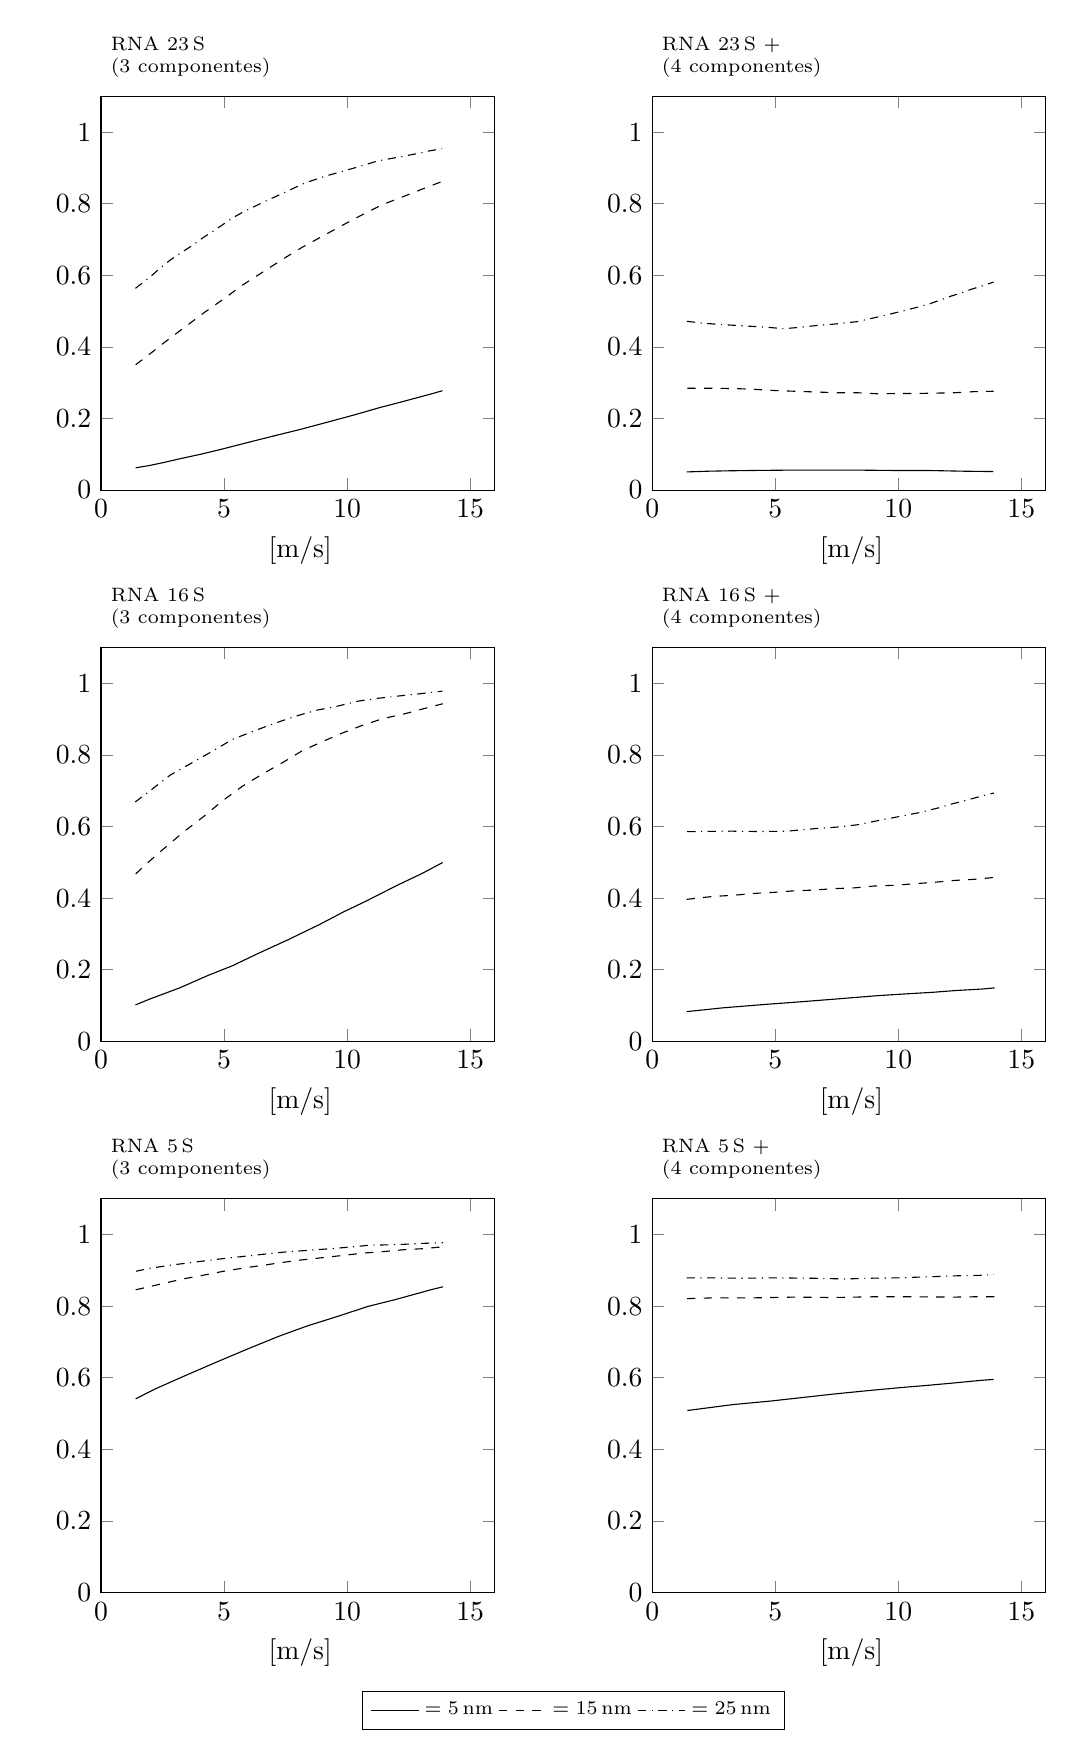
\begin{tikzpicture}

\node[right,align=left,font=\scriptsize] at (0cm,19.5cm) {RNA 23\,S\\ (3 componentes)};
\node[right,align=left,font=\scriptsize] at (7cm,19.5cm) {RNA 23\,S + \pVAX \\(4 componentes)};
\node[right,align=left,font=\scriptsize] at (0cm,12.5cm) {RNA 16\,S\\ (3 componentes)};
\node[right,align=left,font=\scriptsize] at (7cm,12.5cm) {RNA 16\,S + \pVAX \\ (4 componentes)};
\node[right,align=left,font=\scriptsize] at (0cm,5.5cm) {RNA 5\,S\\ (3 componentes)};
\node[right,align=left,font=\scriptsize] at (7cm,5.5cm) {RNA 5\,S + \pVAX\\ (4 componentes)};

\begin{axis}[%
%scaled ticks=false,
width=5cm,
height=5cm,
forget plot,
scale only axis,
xmin=0,
xmax=16,
xlabel={\fluxo\,[\micro m/s]},
ymin=0,
ymax=1.1,
ylabel={\permobs},
at={(0cm,14cm)},
anchor=south west
]

\addplot[
color=black,
solid
]
table[row sep=crcr]{
1.4092 0.0622\\
1.9512 0.0684\\
2.5908 0.0777\\
3.2412 0.0881\\
4.0108 0.0995\\
4.8347 0.1130\\
5.8862 0.1316\\
7.0786 0.1523\\
8.0650 0.1689\\
9.0840 0.1876\\
10.255 0.2093\\
11.360 0.2311\\
12.228 0.2466\\
12.900 0.2591\\
13.518 0.2705\\
13.875 0.2777\\
};

\addplot[
color=black,
dashed
]
table[row sep=crcr]{
1.4092 0.3503\\
1.9079 0.3762\\
2.5366 0.4104\\
3.2954 0.4497\\
4.1409 0.4933\\
4.9756 0.5337\\
5.7778 0.5741\\
6.5799 0.6093\\
7.3713 0.6446\\
8.1843 0.6788\\
8.9864 0.7088\\
9.8103 0.7399\\
10.634 0.7699\\
11.447 0.7979\\
12.238 0.8187\\
13.073 0.8415\\
13.897 0.8632\\
};

\addplot[
color=black,
dashdotted
]
table[row sep=crcr]{
1.3984 0.5637\\
1.9729 0.5938\\
2.3740 0.6187\\
2.8076 0.6425\\
3.2304 0.6622\\
3.6748 0.6819\\
4.0867 0.7026\\
4.5095 0.7212\\
4.9106 0.7399\\
5.3550 0.7606\\
5.7778 0.7772\\
6.6233 0.8052\\
7.4472 0.8311\\
8.2818 0.8580\\
9.1491 0.8777\\
10.428 0.9026\\
11.274 0.9202\\
12.130 0.9306\\
12.986 0.9420\\
13.377 0.9482\\
13.864 0.9534\\
};

\end{axis}


\begin{axis}[%
%scaled ticks=false,
width=5cm,
height=5cm,
forget plot,
scale only axis,
xmin=0,
xmax=16,
xlabel={\fluxo\,[\micro m/s]},
ymin=0,
ymax=1.1,
ylabel={\permobs},
at={(7cm,14cm)},
anchor=south west
]

\addplot[
color=black,
solid
]
table[row sep=crcr]{
1.3974 0.0507\\
2.2640 0.0527\\
3.0548 0.0538\\
4.1273 0.0548\\
5.6980 0.0558\\
8.2654 0.0558\\
9.7820 0.0548\\
11.169 0.0548\\
12.685 0.0527\\
13.866 0.0517\\
};

\addplot[
color=black,
dashed
]
table[row sep=crcr]{
1.4299 0.2844\\
1.9066 0.2844\\
2.6324 0.2844\\
3.4665 0.2834\\
4.1706 0.2813\\
4.9614 0.2782\\
5.7955 0.2761\\
6.6622 0.2740\\
7.5179 0.2720\\
8.3304 0.2720\\
9.1862 0.2689\\
10.020 0.2699\\
10.768 0.2699\\
11.537 0.2709\\
12.295 0.2720\\
13.108 0.2751\\
13.877 0.2761\\
};

\addplot[
color=black,
dashdotted
]
table[row sep=crcr]{
1.4083 0.4716\\
2.0366 0.4664\\
2.8490 0.4623\\
3.6290 0.4592\\
4.1381 0.4571\\
4.6581 0.4550\\
5.3406 0.4509\\
5.8822 0.4540\\
6.5972 0.4592\\
7.3230 0.4633\\
8.3196 0.4705\\
9.1212 0.4829\\
9.5762 0.4902\\
10.064 0.4984\\
10.833 0.5119\\
11.266 0.5202\\
11.689 0.5305\\
12.144 0.5419\\
12.534 0.5502\\
12.945 0.5605\\
13.378 0.5698\\
13.877 0.5812\\
};

\end{axis}


\begin{axis}[%
%scaled ticks=false,
width=5cm,
height=5cm,
forget plot,
scale only axis,
xmin=0,
xmax=16,
xlabel={\fluxo\,[\micro m/s]},
ymin=0,
ymax=1.1,
ylabel={\permobs},
at={(0cm,7cm)},
anchor=south west
]

\addplot[
color=black,
solid
]
table[row sep=crcr]{
1.3984 0.1016\\
1.9512 0.1171\\
3.1978 0.1492\\
4.3686 0.1845\\
5.3550 0.2114\\
6.2656 0.2415\\
7.5772 0.2829\\
8.8564 0.3254\\
9.8645 0.3617\\
10.775 0.3917\\
12.022 0.4352\\
13.062 0.4694\\
13.886 0.4995\\
};

\addplot[
color=black,
dashed
]
table[row sep=crcr]{
1.4092 0.4674\\
1.8211 0.4943\\
2.4607 0.5326\\
3.3279 0.5834\\
4.1518 0.6269\\
4.9322 0.6715\\
5.7561 0.7130\\
6.5474 0.7461\\
7.3930 0.7793\\
8.1951 0.8124\\
8.9973 0.8373\\
9.8428 0.8622\\
10.634 0.8829\\
11.458 0.9016\\
12.293 0.9140\\
13.073 0.9285\\
13.886 0.9430\\
};

\addplot[
color=black,
dashdotted
]
table[row sep=crcr]{
1.3875 0.6684\\
1.9621 0.6984\\
2.8184 0.7440\\
3.6748 0.7772\\
4.4986 0.8093\\
5.3442 0.8435\\
6.1897 0.8663\\
7.0461 0.8881\\
7.8916 0.9078\\
8.7263 0.9244\\
9.5827 0.9358\\
10.450 0.9503\\
11.285 0.9585\\
12.119 0.9648\\
12.965 0.9710\\
13.875 0.9782\\
};

\end{axis}


\begin{axis}[%
%scaled ticks=false,
width=5cm,
height=5cm,
forget plot,
scale only axis,
xmin=0,
xmax=16,
xlabel={\fluxo\,[\micro m/s]},
ymin=0,
ymax=1.1,
ylabel={\permobs},
at={(7cm,7cm)},
anchor=south west
]

\addplot[
color=black,
solid
]
table[row sep=crcr]{
1.4003 0.0828\\
2.8440 0.0932\\
4.5047 0.1025\\
5.9267 0.1097\\
7.2836 0.1170\\
9.1398 0.1273\\
10.334 0.1325\\
11.365 0.1366\\
12.353 0.1418\\
13.427 0.1460\\
13.916 0.1491\\
};

\addplot[
color=black,
dashed
]
table[row sep=crcr]{
1.4003 0.3965\\
2.4966 0.4048\\
3.3216 0.4079\\
4.1248 0.4130\\
4.9607 0.4161\\
5.7531 0.4203\\
6.5672 0.4224\\
7.4030 0.4265\\
8.2280 0.4286\\
9.0095 0.4337\\
9.8345 0.4358\\
10.649 0.4400\\
11.463 0.4441\\
12.277 0.4493\\
13.069 0.4524\\
13.883 0.4576\\
};

\addplot[
color=black,
dashdotted
]
table[row sep=crcr]{
1.4220 0.5859\\
1.9322 0.5859\\
3.2130 0.5870\\
4.4505 0.5859\\
5.4925 0.5870\\
6.6323 0.5942\\
7.4790 0.5983\\
8.3148 0.6046\\
9.1289 0.6159\\
9.9973 0.6273\\
10.844 0.6387\\
11.701 0.6532\\
12.147 0.6625\\
12.635 0.6708\\
13.395 0.6853\\
13.894 0.6936\\
};

\end{axis}


\begin{axis}[%
%scaled ticks=false,
width=5cm,
height=5cm,
scale only axis,
xmin=0,
xmax=16,
xlabel={\fluxo\,[\micro m/s]},
ymin=0,
ymax=1.1,
ylabel={\permobs},
at={(0cm,0cm)},
anchor=south west,
legend style={at={(6cm,-1.5cm)},legend columns=-1,anchor=center,font=\scriptsize,draw=black,fill=white,legend cell align=left}
]

\addplot[
color=black,
solid
]
table[row sep=crcr]{
1.4092 0.5409\\
2.1789 0.5679\\
3.2629 0.6010\\
4.5854 0.6404\\
5.9079 0.6788\\
7.1978 0.7150\\
8.4011 0.7451\\
9.6043 0.7710\\
10.840 0.7990\\
11.924 0.8176\\
12.856 0.8352\\
13.453 0.8466\\
13.897 0.8539\\
};
\addlegendentry{$\raioporo=5$\,nm};

\addplot[
color=black,
dashed
]
table[row sep=crcr]{
1.4092 0.8456\\
2.5257 0.8632\\
3.3062 0.8756\\
4.1301 0.8860\\
4.9864 0.8974\\
5.8211 0.9067\\
6.5799 0.9140\\
7.4038 0.9223\\
8.2060 0.9295\\
9.0623 0.9358\\
9.8862 0.9420\\
10.678 0.9482\\
11.469 0.9523\\
12.293 0.9575\\
13.117 0.9606\\
13.908 0.9658\\
};
\addlegendentry{$\raioporo=15$\,nm};

\addplot[
color=black,
dashdotted
]
table[row sep=crcr]{
1.4201 0.8974\\
1.9946 0.9057\\
2.7859 0.9140\\
4.0976 0.9254\\
4.9431 0.9326\\
6.2114 0.9420\\
7.4905 0.9513\\
8.3360 0.9554\\
9.5827 0.9617\\
10.883 0.9699\\
12.119 0.9720\\
12.997 0.9751\\
13.897 0.9772\\
};
\addlegendentry{$\raioporo=25$\,nm};

\end{axis}


\begin{axis}[%
%scaled ticks=false,
width=5cm,
height=5cm,
forget plot,
scale only axis,
xmin=0,
xmax=16,
xlabel={\fluxo\,[\micro m/s]},
ymin=0,
ymax=1.1,
ylabel={\permobs},
at={(7cm,0cm)},
anchor=south west
]

\addplot[
color=black,
solid
]
table[row sep=crcr]{
1.4309 0.5083\\
3.2737 0.5248\\
4.8780 0.5352\\
6.0921 0.5445\\
7.4580 0.5549\\
8.8238 0.5642\\
10.125 0.5725\\
11.209 0.5787\\
12.358 0.5859\\
13.279 0.5921\\
13.875 0.5952\\
};

\addplot[
color=black,
dashed
]
table[row sep=crcr]{
1.4201 0.8209\\
2.4390 0.8230\\
4.0650 0.8230\\
5.7561 0.8251\\
7.3171 0.8240\\
8.9973 0.8261\\
10.645 0.8261\\
12.238 0.8251\\
13.127 0.8261\\
13.908 0.8261\\
};

\addplot[
color=black,
dashdotted
]
table[row sep=crcr]{
1.3984 0.8789\\
2.3631 0.8789\\
3.6423 0.8778\\
4.9648 0.8789\\
6.5908 0.8778\\
7.8699 0.8758\\
8.7480 0.8778\\
9.9837 0.8789\\
10.840 0.8810\\
11.696 0.8830\\
12.575 0.8851\\
13.366 0.8861\\
13.886 0.8882\\
};

\end{axis}

\end{tikzpicture}
	\caption[Valores calculados de \permobs\ das várias espécies de RNA]{Valores calculados de \permobs\ das várias espécies de RNA, obtidos pelos modelos de 3 e 4 componentes para a célula de filtração Amicon 8010, em função do fluxo de permeado. Os cálculos foram efetuados para uma velocidade de agitação de 760\,min$^{-1}$, $[\ce{CH3COOK}]=316$\,mol/m$^{3}$ e $T=298$\,K.}
	\label{fig:2art4}
\end{figure}
\begin{figure}
	\centering
	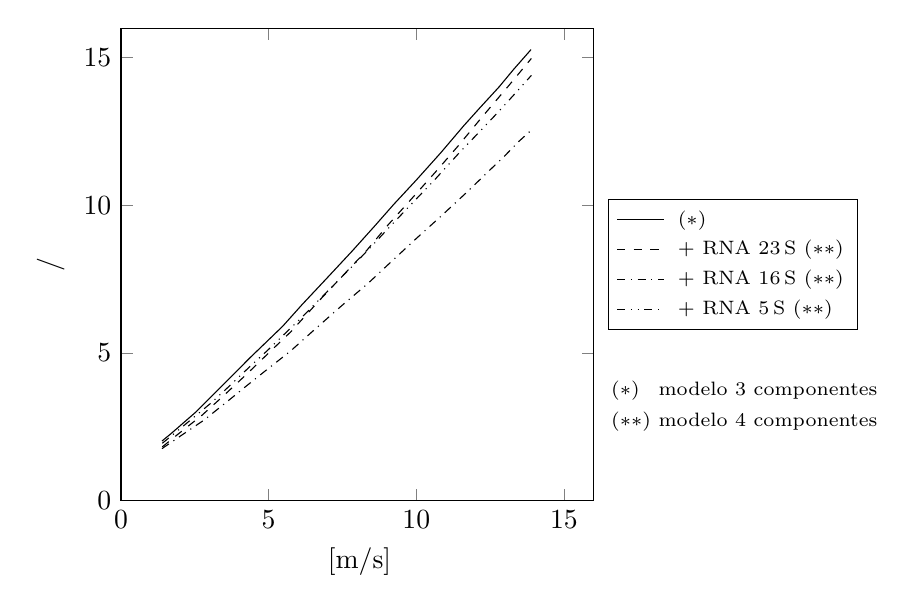
\begin{tikzpicture}

\node[anchor=west,font=\scriptsize] at (6.1cm,1.4cm) {($\ast$)\phantom{$\ast$} modelo 3 componentes};
\node[anchor=west,font=\scriptsize] at (6.1cm,1cm) {($\ast\ast$) modelo 4 componentes};


\begin{axis}[%
width=6cm,
height=6cm,
scale only axis,
xmin=0,
xmax=16,
xlabel={\fluxo\,[\micro m/s]},
ymin=0,
ymax=16,
ylabel={$\concm/\concb$},
at={(0cm,0cm)},
anchor=south west,
legend style={at={(1.03,0.5)},legend columns=1,anchor=west,font=\scriptsize,draw=black,fill=white,legend cell align=left}
]

\addplot[
color=black,
solid
]
table[row sep=crcr]{
1.3875 2.0188\\
1.7344 2.3051\\
2.5474 3.0132\\
3.2087 3.6761\\
4.3794 4.8512\\
5.4743 5.9058\\
6.1355 6.6441\\
6.9702 7.5330\\
7.8266 8.4520\\
8.5854 9.2957\\
9.2358 10.034\\
10.005 10.863\\
10.829 11.782\\
11.610 12.701\\
12.152 13.303\\
12.802 14.011\\
13.290 14.599\\
13.886 15.277\\
};
\addlegendentry{\pVAX\ ($\ast$)};

\addplot[
color=black,
dashed
]
table[row sep=crcr]{
1.3984 1.8230\\
1.9404 2.2599\\
2.7425 2.8927\\
3.4255 3.5104\\
4.2818 4.3089\\
4.9539 4.9567\\
5.7561 5.7250\\
6.6883 6.7495\\
7.5989 7.7137\\
8.3144 8.4670\\
9.0190 9.3107\\
9.8320 10.215\\
10.667 11.149\\
11.425 12.023\\
12.260 13.032\\
13.106 14.026\\
13.897 14.976\\
};
\addlegendentry{\pVAX\ + RNA 23\,S ($\ast\ast$)};

\addplot[
color=black,
dashdotted
]
table[row sep=crcr]{
1.3875 1.7627\\
1.9837 2.1695\\
2.8076 2.7269\\
3.6748 3.4200\\
4.1734 3.8267\\
4.9106 4.4143\\
5.7344 5.0621\\
6.6125 5.8456\\
7.4688 6.5989\\
8.3577 7.3522\\
9.1491 8.0904\\
9.9946 8.8738\\
10.862 9.6573\\
11.707 10.441\\
12.488 11.194\\
13.008 11.691\\
13.463 12.158\\
13.897 12.550\\
};
\addlegendentry{\pVAX\ + RNA 16\,S ($\ast\ast$)};

\addplot[
color=black,
dashdotdotted
]
table[row sep=crcr]{
1.3984 1.9435\\
2.2222 2.6215\\
3.0569 3.3145\\
3.6423 3.8569\\
4.3252 4.5047\\
4.9648 5.0923\\
6.1680 6.2524\\
7.2195 7.3220\\
7.8049 7.9096\\
8.4444 8.5725\\
9.1057 9.2806\\
9.7669 9.9736\\
10.645 10.893\\
11.469 11.797\\
12.065 12.414\\
12.737 13.122\\
13.398 13.846\\
13.897 14.403\\
};
\addlegendentry{\pVAX\ + RNA 5\,S ($\ast\ast$)};

\end{axis}

\end{tikzpicture}
	\caption[Polarização de concentração estimada para o plasmídeo \pVAX]{Polarização de concentração estimada, expressa pelo rácio $\concm/\concb$, para o plasmídeo \pVAX, em função do fluxo de permeado. Cálculos feitos com os modelos de 3 e 4 componentes, para a célula de filtração Amicon 8010, com $\raioporo=5$\,nm, $\agitacao=760$\,min$^{-1}$ e $[\ce{CH3COOK}]=316$\,mol/m$^{3}$.}
	\label{fig:3aart4}
\end{figure}
\begin{figure}
	\centering
	\begin{tikzpicture}

\node[right,font=\scriptsize] at (0cm,12.5cm) {RNA 23\,S};
\node[right,font=\scriptsize] at (7cm,12.5cm) {RNA 16\,S};
\node[right,font=\scriptsize] at (0cm,5.5cm) {RNA 5\,S};

\begin{axis}[%
width=5cm,
height=5cm,
forget plot,
scale only axis,
xmin=0,
xmax=16,
xlabel={\fluxo\,[\micro m/s]},
ymin=0,
ymax=7,
ylabel={$\concm/\concb$},
at={(0cm,7cm)},
anchor=south west
]

\addplot[
color=black,
solid
]
table[row sep=crcr]{
1.3984 1.3697\\
1.9621 1.5409\\
2.8618 1.8241\\
3.9458 2.1994\\
4.9322 2.5484\\
6.0054 2.9172\\
6.7967 3.2267\\
7.7073 3.5823\\
8.4770 3.8655\\
9.2575 4.1881\\
10.038 4.4976\\
10.916 4.8532\\
11.762 5.1891\\
12.336 5.4262\\
12.900 5.6566\\
13.485 5.9003\\
13.886 6.0715\\
};

\addplot[
color=black,
dashed
]
table[row sep=crcr]{
1.3875 1.0865\\
2.3415 1.1261\\
3.2304 1.1590\\
4.0650 1.1656\\
4.9322 1.1787\\
5.7453 1.1919\\
6.6016 1.1853\\
7.4688 1.1919\\
8.7371 1.1853\\
9.5610 1.1853\\
10.407 1.1656\\
11.263 1.1722\\
12.119 1.1458\\
12.943 1.1392\\
13.886 1.1261\\
};

\end{axis}


\begin{axis}[%
width=5cm,
height=5cm,
forget plot,
scale only axis,
xmin=0,
xmax=16,
xlabel={\fluxo\,[\micro m/s]},
ymin=0,
ymax=7,
ylabel={$\concm/\concb$},
at={(7cm,7cm)},
anchor=south west
]

\addplot[
color=black,
solid
]
table[row sep=crcr]{
1.3984 1.3776\\
2.1355 1.6149\\
2.9485 1.8983\\
3.7073 2.1817\\
4.3686 2.4322\\
5.0949 2.7156\\
5.7561 2.9925\\
6.4390 3.2759\\
7.2087 3.6055\\
7.9892 3.9416\\
8.9648 4.3635\\
9.8645 4.7721\\
10.612 5.1083\\
11.480 5.5038\\
12.304 5.8663\\
13.041 6.2090\\
13.875 6.5913\\
};

\addplot[
color=black,
dashed
]
table[row sep=crcr]{
1.3984 1.1139\\
2.0921 1.1601\\
2.7967 1.2194\\
3.6423 1.2853\\
4.9539 1.3842\\
6.1572 1.4765\\
7.4688 1.5621\\
9.0515 1.6610\\
9.9837 1.7269\\
11.263 1.8126\\
12.499 1.8917\\
13.333 1.9510\\
13.875 1.9840\\
};

\end{axis}


\begin{axis}[%
%scaled ticks=false,
width=5cm,
height=5cm,
scale only axis,
xmin=0,
xmax=16,
xlabel={\fluxo\,[\micro m/s]},
ymin=0.8,
ymax=1.8,
ylabel={$\concm/\concb$},
at={(0cm,0cm)},
anchor=south west,
legend style={at={(9.5cm,2.5cm)},legend columns=1,anchor=center,font=\scriptsize,draw=black,fill=white,legend cell align=left,align=left}
]

\addplot[
color=black,
solid
]
table[row sep=crcr]{
1.3993 1.0916\\
2.2237 1.1462\\
3.2325 1.2092\\
4.0353 1.2581\\
4.9247 1.3127\\
5.7275 1.3588\\
6.4976 1.4011\\
7.4522 1.4510\\
8.2766 1.4933\\
9.1336 1.5310\\
9.8495 1.5648\\
10.587 1.5968\\
11.433 1.6297\\
12.236 1.6598\\
13.049 1.6871\\
13.885 1.7172\\
};
\addlegendentry{RNA (3 componentes)};

\addplot[
color=black,
dashed
]
table[row sep=crcr]{
1.3668 1.0239\\
2.3864 1.0408\\
3.6339 1.0606\\
4.5125 1.0747\\
5.3478 1.0869\\
6.5953 1.1048\\
7.4739 1.1170\\
8.7322 1.1340\\
9.6217 1.1452\\
10.457 1.1565\\
11.292 1.1669\\
12.117 1.1763\\
12.616 1.1829\\
13.375 1.1923\\
13.896 1.1970\\
};
\addlegendentry{RNA + \pVAX\\(4 componentes)};

\end{axis}

\end{tikzpicture}
	\caption[Polarização de concentração estimada para as várias espécies de RNA]{Polarização de concentração estimada, expressa pelo rácio $\concm/\concb$, para as várias espécies de RNA, em função do fluxo de permeado. Cálculos feitos com os modelos de 3 e 4 componentes, para a célula de filtração Amicon 8010, com $\raioporo=5$\,nm, $\agitacao=760$\,min$^{-1}$ e $[\ce{CH3COOK}]=316$\,mol/m$^{3}$.}
	\label{fig:3bcdart4}
\end{figure}

Comparando os resultados obtidos para os dois plasmídeos, pode-se observar que, para além do efeito da presença das moléculas de RNA ser semelhante, os valores de \permobs, quer para o plasmídeo \pVAX\ quer para o plasmídeo \pCAMBIA, são semelhantes pese embora os dois plasmídeos apresentem tamanhos distintos, tal como se pode observar na figura~\ref{fig:1dart4}. A independência de \permobs\ com o tamanho das moléculas de pDNA é um resultado previamente reportado na literatura \cite{latu07,latusalt,latu09}. No entanto, deve-se ter especial cuidado na interpretação deste resultado uma vez que, tal como indicado na tabela~\ref{tab:1art4}, as concentrações dos dois plasmídeos nos lisados apresentam quase uma ordem de grandeza de diferença entre si. Sendo moléculas com elevada carga negativa, os efeitos do potencial elétrico na camada de polarização, contabilizados na equação estendida de Nernst-Planck (secção~\ref{sec:ioes}), desempenham um importante papel na permeação deste tipo de biomoléculas. À medida que a concentração de pDNA aumenta é gerado um gradiente do potencial elétrico, de valor negativo, mais acentuado na camada de polarização, facto que leva a uma redução do grau de polarização e consequentemente do valor de \permobs.   

Para se obter uma separação satisfatória entre pDNA e RNA é necessário obter, simultaneamente, valores reduzidos de \permobs\ de pDNA e valores elevados de \permobs\ das moléculas de RNA na operação de ultrafiltração. Dado que a permeação observada das moléculas de RNA é praticamente independente de \fluxo, facto originado pela presença das moléculas de pDNA (ver figura~\ref{fig:2art4}), a utilização de um fluxo elevado não garante por si só uma elevada permeação destas moléculas. Para o conseguir, pode-se optar por utilizar membranas com poros de maiores dimensões (pelo menos de 25\,nm de raio). Assim, considerando que a permeação de pDNA pode ser mantida relativamente baixa aplicando fluxos de filtração de reduzido valor ($1-3$\,\micro m/s) para $\raioporo = 25$\,nm (tal como indicado na figura~\ref{fig:1abcart4}), pode-se concluir que a melhor opção será realizar a operação de ultrafiltração a baixos fluxos e utilizando membranas com $20-25$\,nm de raio de poro.   
% subsection 3.1art4 (end)

\subsection{Resultados experimentais - Ultrafiltração} % (fold)
\label{sub:3.2art4}
\index{ultrafiltração!separação pDNA/RNA}%
Para avaliar as conclusões obtidas, referidas na secção anterior, foram realizados ensaios de ultrafiltração dos lisados microfiltrados de \pVAX\ e \pCAMBIA, utilizando duas membranas distintas, uma com $\raioporo=4.8$\,nm \cite{moraompa} e outra com $\raioporo=25$\,nm, de 100 e 300\,kDa respetivamente, referidas na secção~\ref{ssub:2.3art4}.
\index{pVAX@\pVAX}%
\index{pCAMBIA@\pCAMBIA}%
\index{FS40PP}%
\index{Biomax 300}%
O valor de $\raioporo=25$\,nm foi obtido experimentalmente pela medição das permeações observadas dos dextranos T70 e T500. Foram usadas duas velocidades de agitação (100 e 760\,min$^{-1}$) e diferentes valores de fluxo no intervalo $1.4-8.3$\,\micro m/s ($5-30$\,L/h$\cdot$m$^2$).
\index{dextrano!T70}%
\index{dextrano!T500}%

Os resultados obtidos, para um fator de concentração volumétrico (VCF) igual a 10, estão representados na figura~\ref{fig:4art4}.
\index{fator!de concentração}%
O rendimento de recuperação de pDNA foi calculado como o rácio entre a quantidade de pDNA presente no volume total de permeado recolhido e a quantidade de pDNA presente no volume de permeado da operação de microfiltração (MFP) processado em cada ensaio. O rendimento de remoção de RNA foi calculado como $1-(V_{\mr{p}}C_{\mathrm{RNA,p}})/(V_{\mr{MFP}}C_{\mr{RNA,MFP}})$, onde $C_{\mathrm{RNA,p}}$ representa a concentração no volume total de permeado, $C_{\mr{RNA,MFP}}$ é a concentração de RNA no MFP, $V_{\mr{p}}$ é o volume de permeado recolhido e $V_{\mr{MFP}}$ é o volume de MFP processado em cada ensaio.
\index{MFP}%
\begin{figure}[!t]
	\centering
	\begin{tikzpicture}

\node[right,font=\scriptsize,align=left] at (0cm,12.5cm) {\pVAX\\$\raioporo=4.8$\,nm, $\agitacao=100$\,min$^{-1}$};
\node[right,font=\scriptsize,align=left] at (7cm,12.5cm) {\pVAX\\$\raioporo=4.8$\,nm, $\agitacao=760$\,min$^{-1}$};
\node[right,font=\scriptsize,align=left] at (0cm,5.5cm) {\pVAX\\$\raioporo=25$\,nm, $\agitacao=760$\,min$^{-1}$};
\node[right,font=\scriptsize,align=left] at (7cm,5.5cm) {\pCAMBIA\\$\raioporo=25$\,nm, $\agitacao=760$\,min$^{-1}$};

\begin{axis}[%
width=5cm,
height=5cm,
forget plot,
scale only axis,
xmin=0,
xmax=20,
xlabel={\fluxo\,[\micro m/s]},
ymin=-0.1,
ymax=1.1,
ylabel={Rend. pDNA ou Remo. RNA},
at={(0cm,7cm)},
anchor=south west
]

\addplot[
color=black,
mark=*,
only marks,
mark options={solid,fill=black,draw=black}
]
plot [error bars/.cd, y dir = both, y explicit]
coordinates{
(3.909,1.023) +- (0.000,0.052)
(8.117,1.008) +- (0.000,0.049)
(16.25,0.802) +- (0.000,0.078)
};

\addplot[
color=black,
solid
]
table[row sep=crcr]{
1.4184 0.9755\\
2.4271 0.9644\\
4.4129 0.9388\\
5.9417 0.9187\\
7.3444 0.8987\\
9.0623 0.8753\\
10.701 0.8530\\
12.151 0.8318\\
13.790 0.8085\\
14.878 0.7929\\
15.745 0.7817\\
16.675 0.7695\\
};

\addplot[%0.5MIC
color=black,
mark=*,
only marks,
mark options={solid,fill=white,draw=black}
]
plot [error bars/.cd, y dir = both, y explicit]
coordinates{
(3.893,0.187) +- (0.000,0.080)
(8.117,0.334	) +- (0.000,0.102)
(16.26,0.369) +- (0.000,0.090)
};

\addplot[
color=black,
dashed
]
table[row sep=crcr]{
1.4184 0.3641\\
2.3325 0.3753\\
3.4515 0.3898\\
4.6966 0.4031\\
5.8629 0.4154\\
7.1080 0.4243\\
8.4003 0.4365\\
9.5981 0.4443\\
10.875 0.4521\\
12.025 0.4588\\
13.302 0.4655\\
14.500 0.4710\\
15.713 0.4777\\
16.548 0.4788\\
};

\end{axis}


\begin{axis}[%
width=5cm,
height=5cm,
forget plot,
scale only axis,
xmin=0,
xmax=20,
xlabel={\fluxo\,[\micro m/s]},
ymin=-0.1,
ymax=1.1,
ylabel={Rend. pDNA ou Remo. RNA},
at={(7cm,7cm)},
anchor=south west
]

\addplot[
color=black,
mark=*,
only marks,
mark options={solid,fill=black,draw=black}
]
plot [error bars/.cd, y dir = both, y explicit]
coordinates{
(4.063,0.969) +- (0.000,0.050)
(8.126,1.030) +- (0.000,0.048)
(16.25,0.997) +- (0.000,0.093)
};

\addplot[
color=black,
solid
]
table[row sep=crcr]{
1.4331 0.9878\\
2.8346 0.9811\\
4.7244 0.9745\\
6.6614 0.9678\\
8.5039 0.9600\\
10.094 0.9534\\
11.843 0.9467\\
13.276 0.9390\\
14.677 0.9356\\
15.827 0.9290\\
16.646 0.9256\\
};

\addplot[%0.5MIC
color=black,
mark=*,
only marks,
mark options={solid,fill=white,draw=black}
]
plot [error bars/.cd, y dir = both, y explicit]
coordinates{
(4.063,0.090) +- (0.000,0.054)
(8.142,0.139) +- (0.000,0.032)
(16.27,0.161) +- (0.000,0.041)
};

\addplot[
color=black,
dashed
]
table[row sep=crcr]{
1.3858 0.3507\\
2.8976 0.3585\\
4.5984 0.3663\\
5.9213 0.3718\\
7.5906 0.3774\\
8.9134 0.3829\\
10.772 0.3907\\
12.520 0.3973\\
13.858 0.4018\\
15.118 0.4051\\
16.583 0.4084\\
};

\end{axis}


\begin{axis}[%
width=5cm,
height=5cm,
scale only axis,
xmin=0,
xmax=20,
xlabel={\fluxo\,[\micro m/s]},
ymin=-0.1,
ymax=1.1,
ylabel={Rend. pDNA ou Remo. RNA},
at={(0cm,0cm)},
anchor=south west,
legend style={at={(6cm,-2cm)},legend columns=2,anchor=center,font=\scriptsize,draw=black,fill=white,legend cell align=left}
]

\addplot[
color=black,
mark=*,
only marks,
mark options={solid,fill=black,draw=black}
]
plot [error bars/.cd, y dir = both, y explicit]
coordinates{
(1.290,0.900) +- (0.000,0.080)
(2.486,0.931) +- (0.000,0.081)
(4.028,0.806) +- (0.000,0.057)
(8.749,0.412) +- (0.000,0.068)
};\addlegendentry{Rendimento de pDNA (exp)};

\addplot[
color=black,
solid
]
table[row sep=crcr]{
1.3847 0.7389\\
1.9984 0.7011\\
3.0999 0.6322\\
4.3745 0.5556\\
5.6491 0.4822\\
6.5460 0.4322\\
7.9780 0.3556\\
9.1424 0.3011\\
10.212 0.2533\\
11.377 0.2056\\
12.258 0.1767\\
13.108 0.1567\\
13.895 0.1389\\
};\addlegendentry{Rendimento de pDNA (teo)};

\addplot[%0.5MIC
color=black,
mark=*,
only marks,
mark options={solid,fill=white,draw=black}
]
plot [error bars/.cd, y dir = both, y explicit]
coordinates{
(1.259,0.763) +- (0.000,0.049)
(2.502,0.879) +- (0.000,0.088)
(4.028,0.879) +- (0.000,0.090)
(8.718,0.816) +- (0.000,0.073)
};\addlegendentry{Remoção de RNA (exp)}

\addplot[
color=black,
dashed
]
table[row sep=crcr]{
1.4005 0.7489\\
2.8167 0.7411\\
4.6105 0.7367\\
5.8222 0.7344\\
7.1125 0.7389\\
8.2455 0.7400\\
9.5515 0.7478\\
10.291 0.7533\\
11.393 0.7589\\
12.179 0.7678\\
12.777 0.7711\\
13.375 0.7778\\
13.879 0.7822\\
};\addlegendentry{Remoção de RNA (teo)}

\end{axis}


\begin{axis}[%
width=5cm,
height=5cm,
forget plot,
scale only axis,
xmin=0,
xmax=20,
xlabel={\fluxo\,[\micro m/s]},
ymin=-0.1,
ymax=1.1,
ylabel={Rend. pDNA ou Remo. RNA},
at={(7cm,0cm)},
anchor=south west
]

\addplot[
color=black,
mark=*,
only marks,
mark options={solid,fill=black,draw=black}
]
plot [error bars/.cd, y dir = both, y explicit]
coordinates{
(2.423,0.992) +- (0.000,0.047)
(4.296,0.933) +- (0.000,0.093)
(8.765,0.412) +- (0.000,0.083)
};

\addplot[
color=black,
solid
]
table[row sep=crcr]{
1.4005 0.8322\\
2.2659 0.7722\\
3.0685 0.7167\\
3.8238 0.6611\\
4.5633 0.6067\\
5.3659 0.5489\\
6.3415 0.4822\\
7.2541 0.4200\\
8.3399 0.3456\\
9.1739 0.2956\\
10.165 0.2378\\
11.046 0.1900\\
12.006 0.1533\\
12.825 0.1311\\
13.548 0.1178\\
13.863 0.1122\\
};

\addplot[%0.5MIC
color=black,
mark=*,
only marks,
mark options={solid,fill=white,draw=black}
]
plot [error bars/.cd, y dir = both, y explicit]
coordinates{
(2.423,0.892) +- (0.000,0.039)
(4.296,0.788) +- (0.000,0.063)
(8.765,0.821) +- (0.000,0.046)
};

\addplot[
color=black,
dashed
]
table[row sep=crcr]{
1.4162 0.7544\\
2.8482 0.7533\\
4.7364 0.7511\\
5.9481 0.7511\\
7.0653 0.7533\\
8.3714 0.7556\\
10.165 0.7656\\
11.487 0.7722\\
12.667 0.7833\\
13.895 0.7933\\
};

\end{axis}

\end{tikzpicture}

	\caption[Rendimentos de recuperação de pDNA e rendimentos de remoção de RNA (exp.)]{Rendimentos de recuperação de pDNA e rendimentos de remoção de RNA, determinados experimentalmente, comparados com as previsões teóricas para o processo de filtração (concentração do MFP com duas membranas distintas a VCF=10). Na figura está igualmente indicado o raio do poro e a velocidade de agitação usada em cada ensaio.}
	\label{fig:4art4}
\end{figure}

Como se pode verificar na figura~\ref{fig:4art4}, a utilização da membrana com $\raioporo=25$\,nm, a baixos fluxos de filtração, é claramente a melhor opção para obter, simultaneamente, um elevado rendimento de recuperação de pDNA e um elevado rendimento de remoção de RNA. Para a membrana com $\raioporo=4.8$\,nm, a remoção do RNA 23S e 16S é reduzida, tal como se pode constatar pela análise da figura~\ref{fig:5art4}. Para a membrana com $\raioporo=25$\,nm observa-se uma elevada permeação de todas as espécies de RNA (figura~\ref{fig:5art4}), em todo o intervalo de fluxos considerados nos ensaios, no entanto, só para valores reduzidos de fluxo se consegue obter um elevado rendimento de recuperação de pDNA. 
\begin{figure}[!t]
	\centering
	%!TEX root=tese.tex
\begin{tikzpicture}

\node[right,font=\scriptsize,align=left] at (0cm,12.5cm) {RNA + \pVAX\\$\raioporo=4.8$\,nm, $\agitacao=100$\,min$^{-1}$}; 
\node[right,font=\scriptsize,align=left] at (7cm,12.5cm) {RNA + \pVAX\\$\raioporo=4.8$\,nm, $\agitacao=760$\,min$^{-1}$}; 
\node[right,font=\scriptsize,align=left] at (0cm,5.5cm) {RNA + \pVAX\\$\raioporo=25$\,nm, $\agitacao=760$\,min$^{-1}$}; 
\node[right,font=\scriptsize,align=left] at (7cm,5.5cm) {RNA + \pCAMBIA\\$\raioporo=25$\,nm, $\agitacao=760$\,min$^{-1}$}; 


\begin{axis}[%
width=5cm,
height=5cm,
forget plot,
scale only axis,
xmin=0,
xmax=18,
xlabel={\fluxo\,[\micro m/s]},
ymin=0,
ymax=1,
ylabel={Remoção RNA},
at={(0cm,7cm)},
anchor=south west
]

\addplot[
color=black,
solid
]
table[row sep=crcr]{
1.4146 0.0847\\
2.2927 0.0809\\
3.5610 0.0771\\
4.7439 0.0724\\
5.8293 0.0696\\
7.0000 0.0649\\
8.0976 0.0602\\
9.3171 0.0555\\
10.732 0.0508\\
11.707 0.0480\\
12.756 0.0442\\
14.037 0.0423\\
15.207 0.0395\\
16.085 0.0367\\
16.634 0.0357\\
};

\addplot[
color=black,
dashed
]
table[row sep=crcr]{
1.4268 0.1590\\
1.9878 0.1722\\
2.7195 0.1872\\
3.6098 0.2051\\
4.5244 0.2239\\
5.4512 0.2408\\
6.3415 0.2578\\
7.2927 0.2766\\
8.2561 0.2935\\
9.1585 0.3086\\
10.134 0.3227\\
11.000 0.3377\\
11.902 0.3500\\
12.902 0.3622\\
13.768 0.3754\\
14.720 0.3857\\
15.671 0.3960\\
16.671 0.4064\\
};

\addplot[
color=black,
dashdotted
]
table[row sep=crcr]{
1.4024 0.6576\\
2.0610 0.6707\\
3.0976 0.6867\\
3.9390 0.6971\\
5.2683 0.7159\\
6.3049 0.7262\\
7.2927 0.7357\\
8.2561 0.7451\\
9.1098 0.7526\\
10.146 0.7592\\
11.049 0.7658\\
12.000 0.7714\\
12.939 0.7770\\
13.976 0.7827\\
14.817 0.7865\\
15.793 0.7893\\
16.671 0.7930\\
};

\end{axis}


\begin{axis}[%
width=5cm,
height=5cm,
forget plot,
scale only axis,
xmin=0,
xmax=18,
xlabel={\fluxo\,[\micro m/s]},
ymin=0,
ymax=1,
ylabel={Remoção RNA},
at={(7cm,7cm)},
anchor=south west
]

\addplot[
color=black,
solid
]
table[row sep=crcr]{
1.4146 0.0838\\
2.5488 0.0829\\
3.5732 0.0829\\
4.9146 0.0829\\
6.1585 0.0838\\
7.2805 0.0838\\
8.3902 0.0819\\
9.5610 0.0810\\
10.707 0.0791\\
11.963 0.0782\\
13.159 0.0763\\
14.488 0.0744\\
15.585 0.0734\\
16.695 0.0716\\
};

\addplot[
color=black,
dashed
]
table[row sep=crcr]{
1.4146 0.1384\\
2.1829 0.1441\\
3.4146 0.1535\\
4.6585 0.1629\\
5.5854 0.1685\\
6.5000 0.1751\\
7.4390 0.1798\\
8.2805 0.1855\\
9.1951 0.1921\\
10.085 0.1959\\
11.000 0.2043\\
12.012 0.2100\\
12.878 0.2156\\
13.793 0.2213\\
14.841 0.2279\\
15.756 0.2345\\
16.683 0.2392\\
};

\addplot[
color=black,
dashdotted
]
table[row sep=crcr]{
1.4268 0.6412\\
2.5244 0.6488\\
3.4024 0.6535\\
4.4146 0.6591\\
5.5000 0.6657\\
6.7805 0.6723\\
7.8171 0.6780\\
9.2683 0.6846\\
10.134 0.6902\\
11.134 0.6940\\
12.110 0.6977\\
13.049 0.7024\\
13.951 0.7062\\
14.939 0.7109\\
15.780 0.7128\\
16.671 0.7175\\
};

\end{axis}


\begin{axis}[%
width=5cm,
height=5cm,
scale only axis,
xmin=0,
xmax=16,
xlabel={\fluxo\,[\micro m/s]},
ymin=0,
ymax=1,
ylabel={Remoção RNA},
at={(0cm,0cm)},
anchor=south west,
legend style={at={(6cm,-1.5cm)},legend columns=-1,anchor=center,font=\scriptsize,draw=black,fill=white,legend cell align=left}
]

\addplot[
color=black,
solid
]
table[row sep=crcr]{
1.3984 0.6096\\
2.2439 0.5974\\
3.1111 0.5889\\
3.9350 0.5823\\
4.8238 0.5776\\
5.4634 0.5757\\
6.3523 0.5748\\
7.0027 0.5767\\
7.7507 0.5823\\
8.4661 0.5880\\
9.4851 0.6002\\
10.266 0.6105\\
10.992 0.6218\\
11.772 0.6331\\
12.401 0.6453\\
12.976 0.6557\\
13.474 0.6642\\
13.886 0.6717\\
};
\addlegendentry{RNA 23\,S};

\addplot[
color=black,
dashed
]
table[row sep=crcr]{
1.4201 0.7018\\
1.9404 0.6990\\
2.5691 0.6961\\
3.4580 0.6943\\
4.1951 0.6924\\
4.9864 0.6914\\
5.7236 0.6914\\
6.6016 0.6933\\
7.3604 0.6961\\
8.2276 0.7008\\
9.1057 0.7065\\
9.8428 0.7121\\
10.623 0.7206\\
11.415 0.7281\\
12.271 0.7385\\
12.997 0.7469\\
13.680 0.7554\\
13.886 0.7592\\
};
\addlegendentry{RNA 16\,S};

\addplot[
color=black,
dashdotted
]
table[row sep=crcr]{
1.4092 0.8617\\
2.1138 0.8598\\
2.9268 0.8598\\
4.0217 0.8589\\
4.8238 0.8589\\
5.8753 0.8589\\
7.0678 0.8579\\
7.8808 0.8579\\
8.9431 0.8589\\
10.168 0.8589\\
11.469 0.8598\\
12.228 0.8617\\
13.344 0.8617\\
13.875 0.8636\\
};
\addlegendentry{RNA 5\,S};

\end{axis}


\begin{axis}[%
width=5cm,
height=5cm,
forget plot,
scale only axis,
xmin=0,
xmax=16,
xlabel={\fluxo\,[\micro m/s]},
ymin=0,
ymax=1,
ylabel={Remoção RNA},
at={(7cm,0cm)},
anchor=south west
]

\addplot[
color=black,
solid
]
table[row sep=crcr]{
1.3974 0.6252\\
2.1124 0.6215\\
3.0440 0.6168\\
3.8565 0.6139\\
4.9397 0.6111\\
5.7630 0.6102\\
6.5538 0.6102\\
7.3879 0.6139\\
8.3846 0.6196\\
9.1645 0.6271\\
9.7820 0.6337\\
10.724 0.6450\\
11.494 0.6554\\
12.165 0.6657\\
12.913 0.6780\\
13.433 0.6864\\
13.898 0.6949\\
};

\addplot[
color=black,
dashed
]
table[row sep=crcr]{
1.4191 0.7119\\
1.9282 0.7109\\
3.1523 0.7109\\
4.0298 0.7100\\
4.8964 0.7100\\
5.8497 0.7128\\
6.7163 0.7147\\
7.6371 0.7166\\
8.3629 0.7213\\
9.2620 0.7269\\
10.042 0.7316\\
10.854 0.7392\\
11.678 0.7458\\
12.360 0.7542\\
13.075 0.7618\\
13.898 0.7712\\
};

\addplot[
color=black,
dashdotted
]
table[row sep=crcr]{
1.4191 0.8606\\
2.1774 0.8606\\
2.9898 0.8606\\
4.0948 0.8606\\
5.2539 0.8606\\
6.5322 0.8606\\
7.7671 0.8616\\
9.0670 0.8606\\
10.237 0.8606\\
11.461 0.8616\\
12.696 0.8625\\
13.465 0.8635\\
13.877 0.8644\\
};

\end{axis}

\end{tikzpicture}
	\caption[Valores calculados de remoção de RNA no processo de ultrafiltração]{Valores calculados de remoção de RNA no processo de ultrafiltração estudado (concentração do MFP com duas membranas distintas, a $\mr{VCF}=10$). Na figura está igualmente indicado o tamanho de poro e a velocidade de agitação utilizada em cada ensaio.}
	\label{fig:5art4}
\end{figure}

Para comparar os resultados experimentais com as previsões do modelo, efetuaram-se os cálculos do rendimento de recuperação de pDNA e do rendimento de remoção de RNA através dos modelos de 3 e 4 componentes, respetivamente, uma vez que a presença das moléculas de RNA apresenta uma reduzida influência na permeação de pDNA. Os valores de remoção total de RNA, indicados na figura~\ref{fig:4art4}, foram obtidos a partir das concentrações iniciais de cada tipo de RNA (tabela~\ref{tab:1art4}) e da remoção estimada das diferentes espécies de RNA, indicada na figura~\ref{fig:5art4}. Como se pode constatar na figura~\ref{fig:4art4}, as previsões da remoção de RNA total estão de acordo com os resultados experimentais, embora se observe uma ligeira tendência para se verificarem rendimentos de recuperação de pDNA mais altos do que o previsto, assim como rendimentos de remoção de RNA total mais reduzidos.
\index{DNA plasmídico!rendimento de recuperação}%
\index{RNA!rendimento de remoção}%
Esta tendência indica que as permeações destas moléculas foram inferiores ao previsto, facto que pode sugerir alguma ocorrência de colmatação. 

O sucesso da aplicação de uma operação de ultrafiltração, para separar pDNA e RNA, com a membrana de 25\,nm foi igualmente testado por eletroforese (figura~\ref{fig:6art4}). Como se pode observar, usando a membrana de 25\,nm (\emph{Biomax 300}) os permeados da ultrafiltração (UFP) contêm quantidades significativas de RNA e simultaneamente reduzidas quantidades de pDNA. Observa-se igualmente uma clara permeação de HMw\,RNA, o que indica que a separação do pDNA, quer do HMw\,RNA quer de LMw\,RNA, pode assim ser obtida. Para a membrana de 4.8\,nm (FS40PP), observa-se um comportamento distinto na medida em que a grande maioria do RNA é retido pela membrana, em especial o HMw\,RNA, o que está de acordo com as previsões do modelo.
\index{RNA!alto peso molecular}%
\index{RNA!baixo peso molecular}%
\index{HMw\,RNA|see{RNA}}%
\index{LMw\,RNA|see{RNA}}%
\begin{figure}
	\centering
	%!TEX root=tese.tex
\begin{tikzpicture}
%\draw[help lines] (-5cm,-4cm) grid (7cm,4cm);
\node at (0cm,0cm) {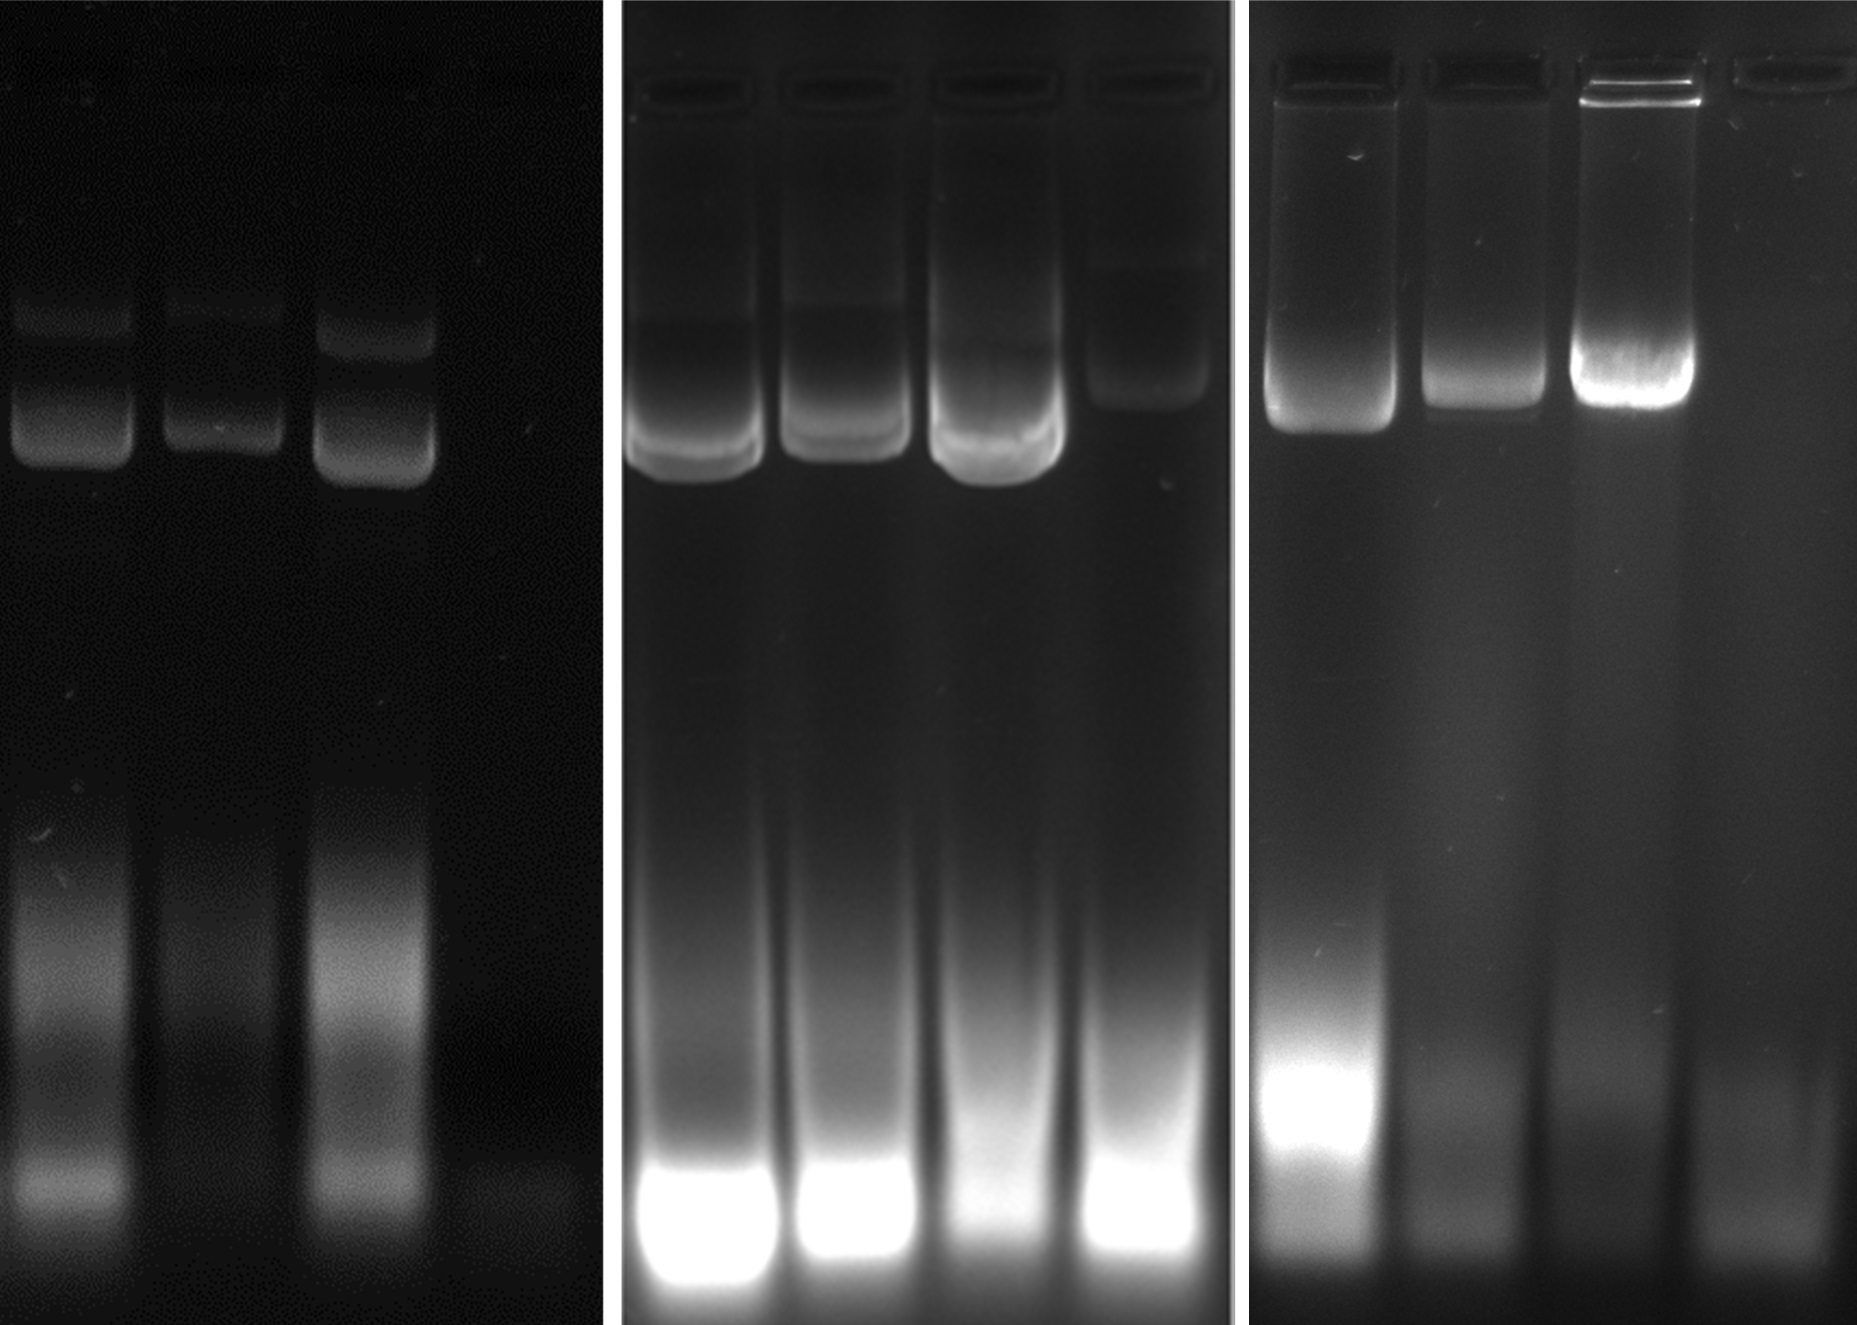
\includegraphics[width=8cm]{EFart4}};

\begin{scope}[font=\scriptsize]
\node[above] at (-3.65cm,2.85cm) {1};
\node[above] at (-3.025cm,2.85cm) {2};
\node[above] at (-2.4cm,2.85cm) {3};
\node[above] at (-1.775cm,2.85cm) {4};

\node[above] at (-1cm,2.85cm) {5};
\node[above] at (-0.375cm,2.85cm) {6};
\node[above] at (0.275cm,2.85cm) {7};
\node[above] at (0.975cm,2.85cm) {8};

\node[above] at (1.75cm,2.85cm) {9};
\node[above] at (2.39cm,2.85cm) {10};
\node[above] at (3.05cm,2.85cm) {11};
\node[above] at (3.725cm,2.85cm) {12};

\draw (4.1,1.35) -- (4.25,1.35) -- (4.35,1.6) -- (4.5,1.6)  node[right,align=left] {\pCAMBIA\\(9--12)};
\draw (4.1,1) -- (4.5,1) node[right,align=left] {\pVAX\\(1--8)};
%\draw (2.6,0.9) -- (3,0.9) node[right] {pDNA (sc)};
\draw (4.1,-1.8) -- (4.5,-1.8) node[right] {HMw\,RNA};
\draw (4.1,-2.5) -- (4.5,-2.5) node[right] {LMw\,RNA};

\end{scope}

\end{tikzpicture}
	\caption[Análise por eletroforese em gel de agarose dos ensaios de ultrafiltração.]{Análise por AGE dos seguintes ensaios: (1--4) MF do lisado da fermentação \pVAX\ seguida de UF a 3.7\,\micro m/s e $\agitacao=760$\,min$^{-1}$, com a membrana \emph{FS40PP} (1-lisado, 2-MFP, 3-UFC, 4-UFC). (5--8) MF do lisado da fermentação do \pVAX\ seguida de UF a 2.4\,\micro m/s e $\agitacao=760$\,min$^{-1}$ com a membrana \emph{Biomax 300} (5-lisado, 6-MFP, 7-UFC, 8-UFP). (9--12) MF do lisado da fermentação com \pCAMBIA\ seguido de UF a 2.4\,\micro m/s e $\agitacao=760$\,min$^{-1}$ com a membrana \emph{Biomax 300} (9-lisado, 10-MFP, 11-UFC, 12-UFP).}
	\label{fig:6art4}
\end{figure}
% subsection 3.2art4 (end)

\subsection{Resultados isolamento intermediário} % (fold)
\label{sub:iso_interm_at4}
\index{isolamento intermediário}%
Os resultados obtidos para os vários processos de isolamento intermediário de pDNA encontram-se na tabela~\ref{tab:res_isol_art4}. Para as condições operatórias escolhidas na realização dos vários ensaios verifica-se uma reduzida colmatação das membranas, colmatação essa representada pelo rácio entre a permeabilidade hidráulica das membranas no fim dos ensaios e as suas permeabilidades iniciais ($L_{\mr{p,f}}/L_{\mr{p},0}$).
\index{permeabilidade hidráulica}%
Este fator pode ter especial importância do ponto de vista de aplicação prática, uma vez que pode proporcionar um aumento no número de ciclos de utilização entre lavagens (ou substituição) de membranas, sendo este parâmetro um dos principais fatores de impacto ambiental e económico deste tipo de processos \cite{freitas}.
\begin{table}[!b]
\centering
	\caption[Resultados obtidos nos processos de isolamento intermediário.]{Resultados obtidos nos vários processos de isolamento intermediário estudados. Os valores encontram-se representados em percentagem com a indicação do respetivo desvio padrão obtido.}
	\label{tab:res_isol_art4}
	\begin{threeparttable}
\begin{tabular*}{0.75\textwidth}{l@{\extracolsep{\fill}} z{2} z{1} z{1} z{3}}
 \toprule
Processo & 
\mc{1}{l}{$L_{\mr{p,f}}/L_{\mr{p},0}$} &
\mc{1}{l}{$R_{\mr{pDNA}}$\tnote{a}} &
\mc{1}{l}{$R_{\mr{RNA}}$\tnote{b}} &
\mc{1}{l}{Pureza\tnote{c}} \\
\midrule
``A'' & 97.3 ? 1.7 & 98.6 ? 3.1 & 19.2 ? 6.1 &  9.53 ? 0.3 \\
``B'' & 87.2 ? 1.6 & 82.1 ? 2.8 & 96.5 ? 1.3 & 63.34 ? 6.1 \\
``C'' & 86.1 ? 1.0 & 95.7 ? 5.0 & 96.6 ? 1.1 & 38.99 ? 2.5 \\
``D'' &            & 88.6 ? 8.0 & 88.0 ? 1.9 & 35.74 ? 2.1 \\
\bottomrule
\end{tabular*}
\begin{tablenotes}
\item[a] Rendimento de recuperação de pDNA  
\item[b] Rendimento de remoção de RNA
\item[c] Pureza cromatográfica nas análises de HIC
\end{tablenotes}
\end{threeparttable}
\end{table}

Com a utilização da membrana com o poro de menores dimensões (FS40PP, Processo A), obtiveram-se elevados rendimentos de recuperação de pDNA, sendo este o processo que apresentou melhor performance neste domínio (tabela~\ref{tab:res_isol_art4}). No entanto, o rendimento de remoção de RNA obtido foi modesto, estando de acordo com os resultados obtidos no capítulo~\ref{chap:art3}. Contudo, é importante referir que este processo pode ainda assim ser útil no contexto do isolamento intermediário de pDNA, por exemplo em operações de concentração e de troca de tampão, dado os valores elevados de rendimento de recuperação de pDNA obtidos e o reduzido grau de colmatação das membranas verificado nestes ensaios.

Tal como referido anteriormente, para obter rendimentos de remoção de RNA mais elevados é necessário utilizar uma membrana com um poro de maiores dimensões. Assim, foi utilizada uma membrana de 300\,kDa de ``cut-off'' (Biomax\,300, $\raioporo = 25$\,nm). Procurou-se melhorar o valor de remoção de RNA através da utilização de uma operação de diafiltração (Processo B). Tal como se pode verificar na tabela~\ref{tab:res_isol_art4}, por este método obtém-se uma elevada remoção de RNA (cerca de 96.5\%), inclusivamente superior à que se obtém com o processo alternativo estudado (88\%, Processo D).
\index{RNA!rendimento de remoção}%
Contudo, o aumento do tamanho do poro conduz igualmente a uma diminuição do rendimento de recuperação de pDNA, por comparação com o Processo A, que se situou em 82\% neste processo. Este valor encontra-se ainda acima do limite mínimo de rendimento que se considera aceitável para uma operação unitária num processo de produção de pDNA \cite{kepka,smrekar,urthaler2}.
\index{DNA plasmídico!rendimento de recuperação}%
A perda de rendimento verificada deve-se essencialmente à permeação de parte do plasmídeo \pVAX\ na membrana, uma vez que grande parte do pDNA restante foi analisado no permeado (cerca de 14\%, em média, do plasmídeo presente inicialmente). A ocorrência de alguma permeação de pDNA, e concomitante elevada permeação das diferentes espécies de RNA presentes, está explicita na análise por eletroforese em gel de agarose de amostras recolhidas ao longo do processo (figura~\ref{fig:ef_processoB_art4}).
\index{AGE}% 
\begin{figure}[!t]
	\centering
	\begin{tikzpicture}

\node at (3cm, 3cm) {%\includegraphics[width=7cm]{% mudar para 6.3 cm
\includegraphics[width=6cm]{ef_processoB_art4.jpg}};

\fill[white] (-0.2cm, 0cm) rectangle (0.8cm, 5.5cm);
\fill[white] (5cm, 0cm) rectangle (6.1cm, 5.5cm);

\node[above, color = white] at (1.225, 4.9) {1};
\node[above, color = white] at (1.7, 4.9) {2};
\node[above, color = white] at (2.2, 4.9) {3};
\node[above, color = white] at (2.675, 4.9) {4};
\node[above, color = white] at (3.2, 4.9) {5};
\node[above, color = white] at (3.675, 4.9) {6};
\node[above, color = white] at (4.2, 4.9) {7};
\node[above, color = white] at (4.675, 4.9) {8};

\draw (5.1, 3.85) -- (5.5, 3.85) node[right] {pDNA\,(sc)};
\draw (5.1, 4.1) -- (5.25, 4.1) -- (5.35, 4.3) -- (5.5, 4.3) node[right] {pDNA\,(oc)}; 
\draw (5.1, 2.4) -- (5.5, 2.4) node[right] {HMw\,RNA};
\draw (5.1, 1.75) -- (5.5, 1.75) node[right] {LMw\,RNA}; 

% \draw[help lines] (0cm, 0cm) grid (8cm, 6cm);
\useasboundingbox (0cm, 0cm) rectangle (8cm, 6cm);

\end{tikzpicture}
	\caption[Análise de amostras, ao longo do processo B, por eletroforese em gel de agarose.]{Análise de amostras, ao longo do processo B, por eletroforese em gel de agarose. Estão representados os resultados obtidos em duas repetições do processo. Amostras 1 e 5: lisado; Amostras 2 e 6: permeado da microfiltração; Amostras 3 e 7; produto final obtido após diafiltração; Amostras 4 e 8: permeado conjunto da operação de ultrafiltração/diafiltração. Na figura é possível verificar a elevada permeação das várias espécies de RNA bem como alguma permeação do plasmídeo \pVAX.}
	\label{fig:ef_processoB_art4}
\end{figure}
Pode ainda ser acrescentado que este processo permitiu obter um valor de pureza cromatográfica bastante superior, quando comparado com o processo alternativo (Processo D), tal como pode ser observado na tabela~\ref{tab:res_isol_art4} e na figura~\ref{fig:hic_comparacao_art4}.
\index{pureza cromatográfica}%
A pureza cromatográfica foi calculada pelo rácio entre a área do pico referente ao plasmídeo e a área total do cromatograma, nas análises pelo método HIC. Na figura~\ref{fig:hic_comparacao_art4} encontram-se as análises de HIC do produto final dos dois processos. O cromatograma referente ao processo B apresenta uma notória superior remoção de contaminantes e consequentemente um valor mais elevado de pureza cromatográfica.
\begin{figure}[!t]
	\centering
	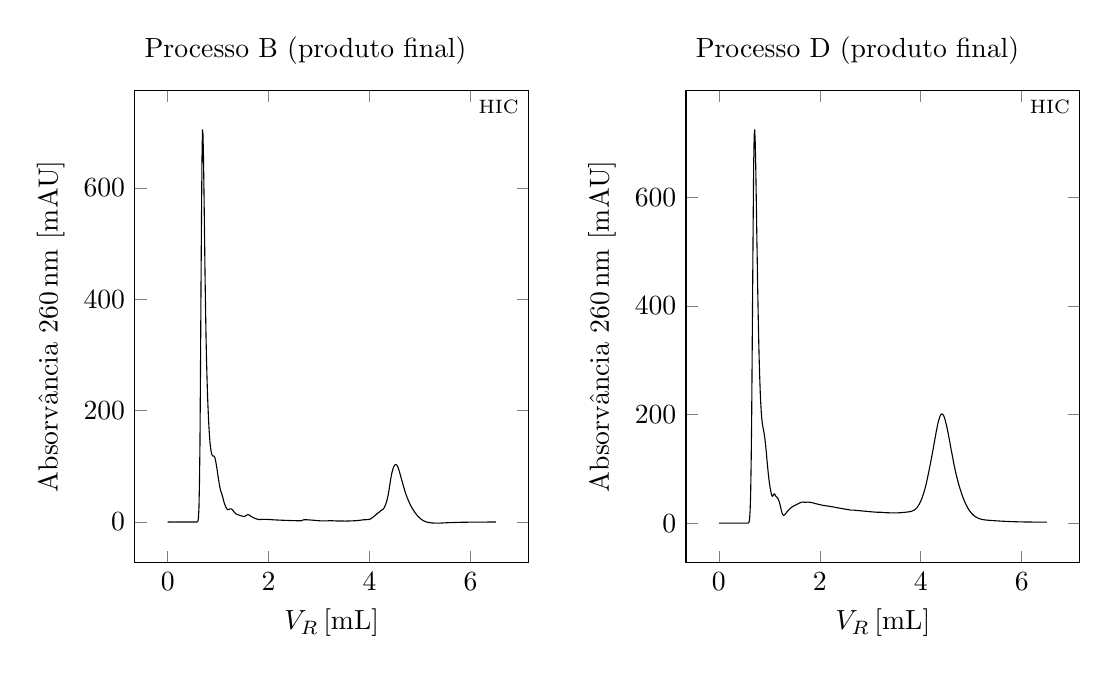
\begin{tikzpicture}

\begin{axis}[%
% xlabel style = {fill = white},
% x tick label style = {fill = white},
width=5cm,
height=6cm,
scale only axis,
% axis y line* = left,
% xmin=-5,
% xmax=85,
xlabel={$V_{\mr{R}}$\,[mL]},
% ymin=-500,
% ymax = 2,
ylabel={Absorvância 260\,nm [mAU]},
at={(0cm, 0cm)},
anchor=south west,
% ylabel near ticks
% legend style={at={(1.03,0.5)},legend columns=1,anchor=west,font=\scriptsize,draw=black,fill=white,legend cell align=left}
]
\addplot[
color=black,
solid
]
table[row sep=crcr]{
0.00000	0.00000\\
0.01000	-0.00319\\
0.02000	-0.00279\\
0.03000	-0.00003\\
0.04000	0.00800\\
0.05000	0.00800\\
0.06000	0.00684\\
0.07000	0.00310\\
0.08000	-0.00503\\
0.09000	-0.01060\\
0.10000	-0.01900\\
0.11000	-0.02172\\
0.12000	-0.02711\\
0.13000	-0.02996\\
0.14000	-0.02740\\
0.15000	-0.01600\\
0.16000	-0.01046\\
0.17000	-0.00101\\
0.18000	0.00385\\
0.19000	0.00287\\
0.20000	0.00900\\
0.21000	0.00102\\
0.22000	0.00243\\
0.23000	0.00360\\
0.24000	0.00708\\
0.25000	0.02400\\
0.26000	0.02072\\
0.27000	0.01969\\
0.28000	0.02318\\
0.29000	0.00789\\
0.30000	0.00888\\
0.31000	0.01552\\
0.32000	0.02325\\
0.33000	0.02541\\
0.34000	0.02423\\
0.35000	0.02292\\
0.36000	0.01889\\
0.37000	0.02303\\
0.38000	0.02763\\
0.39000	0.03353\\
0.40000	0.04330\\
0.41000	0.04494\\
0.42000	0.05299\\
0.43000	0.06001\\
0.44000	0.06100\\
0.45000	0.07314\\
0.46000	0.06984\\
0.47000	0.06196\\
0.48000	0.04930\\
0.49000	0.04746\\
0.50000	0.05140\\
0.51000	0.04581\\
0.52000	0.05822\\
0.53000	0.06233\\
0.54000	0.06167\\
0.55000	0.05450\\
0.56000	0.06139\\
0.57000	0.07566\\
0.58000	0.16256\\
0.59000	0.42631\\
0.60000	1.95446\\
0.61000	8.12856\\
0.62000	25.52763\\
0.63000	69.94649\\
0.64000	140.89924\\
0.65000	269.04561\\
0.66000	414.48015\\
0.67000	545.02997\\
0.68000	653.48344\\
0.69000	705.01673\\
0.70000	696.19861\\
0.71000	651.55936\\
0.72000	590.63611\\
0.73000	520.45869\\
0.74000	445.54502\\
0.75000	386.85822\\
0.76000	331.88873\\
0.77000	290.72830\\
0.78000	256.61163\\
0.79000	226.66150\\
0.80000	205.06388\\
0.81000	183.64954\\
0.82000	167.05330\\
0.83000	153.25521\\
0.84000	141.45760\\
0.85000	133.64444\\
0.86000	127.20937\\
0.87000	123.10997\\
0.88000	120.37367\\
0.89000	118.77187\\
0.90000	118.60709\\
0.91000	118.55548\\
0.92000	117.93753\\
0.93000	116.66145\\
0.94000	114.02649\\
0.95000	109.66127\\
0.96000	104.94424\\
0.97000	99.30794\\
0.98000	93.90067\\
0.99000	87.60856\\
1.00000	81.38730\\
1.01000	75.64406\\
1.02000	69.47163\\
1.03000	64.50407\\
1.04000	60.02512\\
1.05000	56.28509\\
1.06000	53.85458\\
1.07000	51.06158\\
1.08000	47.86160\\
1.09000	44.97569\\
1.10000	41.20834\\
1.11000	37.65127\\
1.12000	34.71720\\
1.13000	32.10887\\
1.14000	29.68245\\
1.15000	27.56398\\
1.16000	25.40531\\
1.17000	23.81828\\
1.18000	23.06117\\
1.19000	22.18864\\
1.20000	22.64264\\
1.21000	22.55848\\
1.22000	22.76408\\
1.23000	23.40284\\
1.24000	23.57731\\
1.25000	23.54345\\
1.26000	23.59975\\
1.27000	23.14316\\
1.28000	22.12947\\
1.29000	21.10960\\
1.30000	20.05726\\
1.31000	18.81123\\
1.32000	17.78075\\
1.33000	16.69056\\
1.34000	15.74811\\
1.35000	15.00334\\
1.36000	14.33357\\
1.37000	13.91543\\
1.38000	13.54449\\
1.39000	13.28825\\
1.40000	13.01713\\
1.41000	12.63920\\
1.42000	12.30297\\
1.43000	11.93290\\
1.44000	11.59175\\
1.45000	11.34565\\
1.46000	11.08482\\
1.47000	10.82204\\
1.48000	10.59200\\
1.49000	10.34684\\
1.50000	10.13829\\
1.51000	10.07100\\
1.52000	10.13183\\
1.53000	10.34814\\
1.54000	10.82641\\
1.55000	11.40114\\
1.56000	12.00786\\
1.57000	12.61584\\
1.58000	13.02598\\
1.59000	13.20546\\
1.60000	13.12087\\
1.61000	12.83750\\
1.62000	12.32358\\
1.63000	11.73703\\
1.64000	11.00704\\
1.65000	10.29940\\
1.66000	9.69510\\
1.67000	9.13187\\
1.68000	8.66831\\
1.69000	8.30152\\
1.70000	7.89327\\
1.71000	7.49074\\
1.72000	7.07692\\
1.73000	6.65769\\
1.74000	6.29790\\
1.75000	5.94366\\
1.76000	5.60424\\
1.77000	5.29557\\
1.78000	5.00575\\
1.79000	4.79466\\
1.80000	4.63104\\
1.81000	4.56859\\
1.82000	4.53370\\
1.83000	4.52477\\
1.84000	4.55740\\
1.85000	4.58895\\
1.86000	4.65239\\
1.87000	4.72644\\
1.88000	4.79895\\
1.89000	4.84448\\
1.90000	4.87022\\
1.91000	4.87427\\
1.92000	4.86187\\
1.93000	4.83097\\
1.94000	4.82099\\
1.95000	4.80904\\
1.96000	4.78674\\
1.97000	4.76374\\
1.98000	4.71430\\
1.99000	4.65011\\
2.00000	4.57981\\
2.01000	4.50510\\
2.02000	4.45320\\
2.03000	4.39894\\
2.04000	4.34534\\
2.05000	4.27717\\
2.06000	4.20933\\
2.07000	4.11948\\
2.08000	4.05992\\
2.09000	4.00561\\
2.10000	3.95988\\
2.11000	3.92508\\
2.12000	3.87424\\
2.13000	3.83032\\
2.14000	3.77495\\
2.15000	3.72877\\
2.16000	3.68692\\
2.17000	3.64255\\
2.18000	3.60118\\
2.19000	3.56594\\
2.20000	3.50460\\
2.21000	3.45769\\
2.22000	3.41567\\
2.23000	3.38039\\
2.24000	3.34236\\
2.25000	3.32477\\
2.26000	3.28807\\
2.27000	3.24316\\
2.28000	3.20442\\
2.29000	3.16406\\
2.30000	3.14202\\
2.31000	3.12577\\
2.32000	3.10121\\
2.33000	3.07144\\
2.34000	3.04011\\
2.35000	2.98315\\
2.36000	2.93968\\
2.37000	2.89214\\
2.38000	2.85858\\
2.39000	2.82993\\
2.40000	2.79946\\
2.41000	2.77372\\
2.42000	2.73963\\
2.43000	2.69805\\
2.44000	2.68058\\
2.45000	2.65845\\
2.46000	2.63724\\
2.47000	2.62007\\
2.48000	2.58733\\
2.49000	2.55330\\
2.50000	2.51948\\
2.51000	2.48068\\
2.52000	2.46078\\
2.53000	2.44331\\
2.54000	2.42252\\
2.55000	2.40547\\
2.56000	2.38328\\
2.57000	2.36654\\
2.58000	2.36145\\
2.59000	2.33838\\
2.60000	2.34639\\
2.61000	2.31576\\
2.62000	2.29207\\
2.63000	2.28277\\
2.64000	2.29608\\
2.65000	2.46760\\
2.66000	2.76167\\
2.67000	3.16447\\
2.68000	3.55412\\
2.69000	3.89542\\
2.70000	4.07660\\
2.71000	4.16248\\
2.72000	4.20010\\
2.73000	4.19282\\
2.74000	4.16519\\
2.75000	4.12419\\
2.76000	4.07371\\
2.77000	4.01668\\
2.78000	3.95456\\
2.79000	3.89149\\
2.80000	3.82833\\
2.81000	3.75442\\
2.82000	3.68804\\
2.83000	3.62076\\
2.84000	3.54983\\
2.85000	3.47941\\
2.86000	3.41364\\
2.87000	3.34973\\
2.88000	3.28613\\
2.89000	3.22421\\
2.90000	3.16082\\
2.91000	3.10042\\
2.92000	3.02966\\
2.93000	2.94451\\
2.94000	2.86216\\
2.95000	2.77067\\
2.96000	2.69081\\
2.97000	2.59595\\
2.98000	2.51150\\
2.99000	2.43694\\
3.00000	2.35344\\
3.01000	2.28912\\
3.02000	2.22104\\
3.03000	2.17172\\
3.04000	2.13077\\
3.05000	2.10550\\
3.06000	2.09381\\
3.07000	2.07932\\
3.08000	2.06688\\
3.09000	2.04627\\
3.10000	2.03125\\
3.11000	2.00600\\
3.12000	2.00251\\
3.13000	1.98645\\
3.14000	1.98271\\
3.15000	2.00273\\
3.16000	2.03123\\
3.17000	2.10707\\
3.18000	2.21989\\
3.19000	2.32294\\
3.20000	2.41643\\
3.21000	2.47721\\
3.22000	2.48459\\
3.23000	2.46117\\
3.24000	2.40479\\
3.25000	2.35822\\
3.26000	2.30255\\
3.27000	2.24843\\
3.28000	2.19948\\
3.29000	2.13964\\
3.30000	2.09073\\
3.31000	2.05307\\
3.32000	2.00626\\
3.33000	1.97273\\
3.34000	1.93367\\
3.35000	1.90875\\
3.36000	1.89557\\
3.37000	1.89337\\
3.38000	1.90407\\
3.39000	1.91539\\
3.40000	1.92419\\
3.41000	1.91021\\
3.42000	1.89760\\
3.43000	1.87660\\
3.44000	1.85253\\
3.45000	1.82824\\
3.46000	1.80228\\
3.47000	1.79405\\
3.48000	1.78278\\
3.49000	1.77345\\
3.50000	1.77057\\
3.51000	1.76248\\
3.52000	1.76096\\
3.53000	1.76517\\
3.54000	1.77464\\
3.55000	1.79440\\
3.56000	1.81054\\
3.57000	1.82904\\
3.58000	1.84705\\
3.59000	1.86491\\
3.60000	1.89725\\
3.61000	1.93743\\
3.62000	1.96374\\
3.63000	2.00504\\
3.64000	2.04833\\
3.65000	2.08834\\
3.66000	2.13421\\
3.67000	2.18709\\
3.68000	2.23058\\
3.69000	2.26622\\
3.70000	2.32402\\
3.71000	2.39094\\
3.72000	2.45459\\
3.73000	2.51906\\
3.74000	2.58221\\
3.75000	2.64627\\
3.76000	2.72471\\
3.77000	2.79790\\
3.78000	2.89682\\
3.79000	2.97547\\
3.80000	3.07014\\
3.81000	3.18751\\
3.82000	3.29545\\
3.83000	3.43502\\
3.84000	3.53800\\
3.85000	3.68840\\
3.86000	3.82627\\
3.87000	3.91215\\
3.88000	4.05097\\
3.89000	4.05901\\
3.90000	4.15232\\
3.91000	4.17164\\
3.92000	4.16251\\
3.93000	4.24416\\
3.94000	4.23491\\
3.95000	4.28271\\
3.96000	4.32541\\
3.97000	4.43170\\
3.98000	4.59979\\
3.99000	4.79163\\
4.00000	5.04350\\
4.01000	5.29676\\
4.02000	5.69280\\
4.03000	6.16688\\
4.04000	6.75612\\
4.05000	7.50441\\
4.06000	8.15056\\
4.07000	8.97493\\
4.08000	9.70150\\
4.09000	10.42212\\
4.10000	11.16584\\
4.11000	11.79421\\
4.12000	12.64509\\
4.13000	13.40227\\
4.14000	14.25354\\
4.15000	15.19466\\
4.16000	15.73232\\
4.17000	16.48164\\
4.18000	17.09590\\
4.19000	17.80193\\
4.20000	18.62849\\
4.21000	19.53557\\
4.22000	20.22566\\
4.23000	20.90787\\
4.24000	21.52656\\
4.25000	22.12303\\
4.26000	22.55921\\
4.27000	23.26982\\
4.28000	24.47958\\
4.29000	25.91480\\
4.30000	27.63320\\
4.31000	29.96465\\
4.32000	32.06548\\
4.33000	34.74787\\
4.34000	37.63365\\
4.35000	41.10140\\
4.36000	45.19253\\
4.37000	49.54535\\
4.38000	54.85259\\
4.39000	60.53994\\
4.40000	66.16454\\
4.41000	72.15323\\
4.42000	77.71702\\
4.43000	82.70860\\
4.44000	87.46207\\
4.45000	91.00652\\
4.46000	94.40213\\
4.47000	97.11617\\
4.48000	99.16921\\
4.49000	101.06455\\
4.50000	102.32452\\
4.51000	103.01482\\
4.52000	103.21476\\
4.53000	102.88253\\
4.54000	102.01101\\
4.55000	100.71815\\
4.56000	98.76823\\
4.57000	96.48269\\
4.58000	93.93680\\
4.59000	90.92388\\
4.60000	87.60919\\
4.61000	84.53308\\
4.62000	81.02874\\
4.63000	77.76603\\
4.64000	74.57315\\
4.65000	71.27362\\
4.66000	68.35089\\
4.67000	65.04720\\
4.68000	61.96309\\
4.69000	58.85874\\
4.70000	55.63381\\
4.71000	52.91539\\
4.72000	50.07222\\
4.73000	47.55988\\
4.74000	45.15644\\
4.75000	42.76165\\
4.76000	40.67474\\
4.77000	38.41351\\
4.78000	36.25217\\
4.79000	34.35585\\
4.80000	32.38986\\
4.81000	30.56755\\
4.82000	28.95376\\
4.83000	27.18077\\
4.84000	25.68802\\
4.85000	24.08466\\
4.86000	22.55590\\
4.87000	21.16442\\
4.88000	19.65941\\
4.89000	18.42333\\
4.90000	17.04910\\
4.91000	15.78362\\
4.92000	14.62056\\
4.93000	13.32487\\
4.94000	12.28534\\
4.95000	11.19995\\
4.96000	10.26399\\
4.97000	9.42838\\
4.98000	8.51727\\
4.99000	7.64440\\
5.00000	6.83945\\
5.01000	5.99580\\
5.02000	5.25097\\
5.03000	4.56911\\
5.04000	3.88284\\
5.05000	3.37127\\
5.06000	2.81764\\
5.07000	2.33053\\
5.08000	1.90527\\
5.09000	1.46590\\
5.10000	1.10800\\
5.11000	0.73184\\
5.12000	0.41717\\
5.13000	0.12073\\
5.14000	-0.19100\\
5.15000	-0.42836\\
5.16000	-0.62051\\
5.17000	-0.78765\\
5.18000	-0.90242\\
5.19000	-1.01362\\
5.20000	-1.19228\\
5.21000	-1.35079\\
5.22000	-1.51336\\
5.23000	-1.61413\\
5.24000	-1.68453\\
5.25000	-1.72327\\
5.26000	-1.73603\\
5.27000	-1.79946\\
5.28000	-1.84925\\
5.29000	-1.89296\\
5.30000	-1.96796\\
5.31000	-2.00622\\
5.32000	-2.03996\\
5.33000	-2.03148\\
5.34000	-2.00886\\
5.35000	-1.99070\\
5.36000	-1.96980\\
5.37000	-1.97376\\
5.38000	-1.96482\\
5.39000	-1.91655\\
5.40000	-1.86026\\
5.41000	-1.83430\\
5.42000	-1.81350\\
5.43000	-1.79188\\
5.44000	-1.73618\\
5.45000	-1.66766\\
5.46000	-1.57019\\
5.47000	-1.50275\\
5.48000	-1.47324\\
5.49000	-1.44965\\
5.50000	-1.42930\\
5.51000	-1.38329\\
5.52000	-1.32752\\
5.53000	-1.27476\\
5.54000	-1.20521\\
5.55000	-1.18050\\
5.56000	-1.16695\\
5.57000	-1.15809\\
5.58000	-1.14435\\
5.59000	-1.13400\\
5.60000	-1.10244\\
5.61000	-1.05576\\
5.62000	-1.03224\\
5.63000	-1.01775\\
5.64000	-0.99700\\
5.65000	-0.96975\\
5.66000	-0.91049\\
5.67000	-0.84752\\
5.68000	-0.79440\\
5.69000	-0.75800\\
5.70000	-0.76238\\
5.71000	-0.75126\\
5.72000	-0.72543\\
5.73000	-0.69923\\
5.74000	-0.65100\\
5.75000	-0.60880\\
5.76000	-0.57952\\
5.77000	-0.54787\\
5.78000	-0.51701\\
5.79000	-0.49300\\
5.80000	-0.47882\\
5.81000	-0.45840\\
5.82000	-0.45457\\
5.83000	-0.44244\\
5.84000	-0.44000\\
5.85000	-0.43919\\
5.86000	-0.43654\\
5.87000	-0.43391\\
5.88000	-0.41182\\
5.89000	-0.37800\\
5.90000	-0.35461\\
5.91000	-0.34370\\
5.92000	-0.33697\\
5.93000	-0.32753\\
5.94000	-0.30600\\
5.95000	-0.27737\\
5.96000	-0.24307\\
5.97000	-0.22623\\
5.98000	-0.23295\\
5.99000	-0.23000\\
6.00000	-0.22717\\
6.01000	-0.21657\\
6.02000	-0.19682\\
6.03000	-0.17877\\
6.04000	-0.16800\\
6.05000	-0.16894\\
6.06000	-0.18215\\
6.07000	-0.19958\\
6.08000	-0.20630\\
6.09000	-0.20300\\
6.10000	-0.18260\\
6.11000	-0.18400\\
6.12000	-0.19313\\
6.13000	-0.19449\\
6.14000	-0.20064\\
6.15000	-0.17438\\
6.16000	-0.15101\\
6.17000	-0.12780\\
6.18000	-0.11683\\
6.19000	-0.10279\\
6.20000	-0.10326\\
6.21000	-0.09238\\
6.22000	-0.08544\\
6.23000	-0.07824\\
6.24000	-0.06232\\
6.25000	-0.04904\\
6.26000	-0.04355\\
6.27000	-0.04388\\
6.28000	-0.03561\\
6.29000	-0.03424\\
6.30000	-0.03977\\
6.31000	-0.03841\\
6.32000	-0.03407\\
6.33000	-0.02986\\
6.34000	-0.02215\\
6.35000	-0.01415\\
6.36000	-0.00641\\
6.37000	-0.00300\\
6.38000	0.01363\\
6.39000	0.01291\\
6.40000	0.00884\\
6.41000	0.01673\\
6.42000	0.02427\\
6.43000	0.05134\\
6.44000	0.07217\\
6.45000	0.08820\\
6.46000	0.10174\\
6.47000	0.10590\\
6.48000	0.10337\\
6.49000	0.10653\\
6.50000	0.11497\\
};
\end{axis}

\begin{axis}[%
% xlabel style = {fill = white},
% x tick label style = {fill = white},
width=5cm,
height=6cm,
scale only axis,
% axis y line* = left,
% xmin=-5,
% xmax=85,
xlabel={$V_{\mr{R}}$\,[mL]},
% ymin=-500,
% ymax = 2,
ylabel={Absorvância 260\,nm [mAU]},
at={(7cm, 0cm)},
anchor=south west,
% ylabel near ticks
% legend style={at={(1.03,0.5)},legend columns=1,anchor=west,font=\scriptsize,draw=black,fill=white,legend cell align=left}
]
\addplot[
color=black,
solid
]
table[row sep=crcr]{
0.00000	-0.00700\\
0.01000	-0.00873\\
0.02000	-0.00696\\
0.03000	0.00249\\
0.04000	0.00929\\
0.05000	0.00400\\
0.06000	0.01167\\
0.07000	0.00462\\
0.08000	-0.00200\\
0.09000	0.00623\\
0.10000	0.00600\\
0.11000	0.00688\\
0.12000	0.01850\\
0.13000	0.02346\\
0.14000	0.02917\\
0.15000	0.03652\\
0.16000	0.03316\\
0.17000	0.03672\\
0.18000	0.03286\\
0.19000	0.02163\\
0.20000	0.02159\\
0.21000	0.00955\\
0.22000	-0.00012\\
0.23000	0.00239\\
0.24000	0.00028\\
0.25000	-0.00100\\
0.26000	0.00034\\
0.27000	-0.00034\\
0.28000	-0.00755\\
0.29000	-0.00617\\
0.30000	-0.00941\\
0.31000	-0.00985\\
0.32000	-0.01210\\
0.33000	-0.01904\\
0.34000	-0.02774\\
0.35000	-0.03103\\
0.36000	-0.03075\\
0.37000	-0.03481\\
0.38000	-0.04208\\
0.39000	-0.04545\\
0.40000	-0.05116\\
0.41000	-0.04763\\
0.42000	-0.03947\\
0.43000	-0.02384\\
0.44000	-0.01466\\
0.45000	-0.01007\\
0.46000	-0.00439\\
0.47000	-0.00706\\
0.48000	-0.00957\\
0.49000	-0.00497\\
0.50000	-0.01141\\
0.51000	-0.01290\\
0.52000	-0.01648\\
0.53000	-0.00861\\
0.54000	-0.01500\\
0.55000	-0.01069\\
0.56000	0.01159\\
0.57000	0.04894\\
0.58000	0.18378\\
0.59000	0.61100\\
0.60000	2.37909\\
0.61000	9.04055\\
0.62000	23.79902\\
0.63000	53.99250\\
0.64000	109.90791\\
0.65000	191.20209\\
0.66000	310.68517\\
0.67000	434.74980\\
0.68000	557.19306\\
0.69000	661.51227\\
0.70000	714.78269\\
0.71000	725.42193\\
0.72000	703.26391\\
0.73000	662.68690\\
0.74000	605.87336\\
0.75000	544.09205\\
0.76000	488.54387\\
0.77000	429.63476\\
0.78000	381.72000\\
0.79000	336.33798\\
0.80000	298.30458\\
0.81000	268.65373\\
0.82000	241.11600\\
0.83000	221.49314\\
0.84000	205.29036\\
0.85000	193.36954\\
0.86000	185.03668\\
0.87000	178.98529\\
0.88000	173.55717\\
0.89000	169.16855\\
0.90000	163.53787\\
0.91000	157.07783\\
0.92000	149.48168\\
0.93000	140.10797\\
0.94000	130.88085\\
0.95000	119.99089\\
0.96000	109.89251\\
0.97000	100.27925\\
0.98000	90.65280\\
0.99000	82.15819\\
1.00000	75.45313\\
1.01000	68.66970\\
1.02000	63.24337\\
1.03000	58.25521\\
1.04000	53.91932\\
1.05000	51.21372\\
1.06000	49.54607\\
1.07000	50.17788\\
1.08000	51.96600\\
1.09000	53.19993\\
1.10000	53.89093\\
1.11000	52.85703\\
1.12000	51.17828\\
1.13000	49.48499\\
1.14000	48.54685\\
1.15000	47.68732\\
1.16000	46.52343\\
1.17000	45.59597\\
1.18000	43.50301\\
1.19000	41.13944\\
1.20000	38.35003\\
1.21000	34.73732\\
1.22000	30.87917\\
1.23000	26.95239\\
1.24000	22.89586\\
1.25000	19.43877\\
1.26000	16.98642\\
1.27000	15.23673\\
1.28000	14.54185\\
1.29000	14.63769\\
1.30000	15.14816\\
1.31000	15.99996\\
1.32000	17.08131\\
1.33000	18.29304\\
1.34000	19.43757\\
1.35000	20.71154\\
1.36000	21.84233\\
1.37000	22.95613\\
1.38000	24.04970\\
1.39000	24.98286\\
1.40000	25.93809\\
1.41000	26.75627\\
1.42000	27.55533\\
1.43000	28.37639\\
1.44000	29.04347\\
1.45000	29.72952\\
1.46000	30.38150\\
1.47000	30.89602\\
1.48000	31.42232\\
1.49000	31.91517\\
1.50000	32.39417\\
1.51000	32.91524\\
1.52000	33.37744\\
1.53000	33.86454\\
1.54000	34.33241\\
1.55000	34.73733\\
1.56000	35.19138\\
1.57000	35.63412\\
1.58000	36.08825\\
1.59000	36.58560\\
1.60000	37.07608\\
1.61000	37.54729\\
1.62000	37.96614\\
1.63000	38.27716\\
1.64000	38.56372\\
1.65000	38.74689\\
1.66000	38.84674\\
1.67000	38.88093\\
1.68000	38.76210\\
1.69000	38.63230\\
1.70000	38.50331\\
1.71000	38.46146\\
1.72000	38.50876\\
1.73000	38.55796\\
1.74000	38.63335\\
1.75000	38.65625\\
1.76000	38.66392\\
1.77000	38.64213\\
1.78000	38.62306\\
1.79000	38.59285\\
1.80000	38.48769\\
1.81000	38.38593\\
1.82000	38.23477\\
1.83000	38.04029\\
1.84000	37.85745\\
1.85000	37.63212\\
1.86000	37.43348\\
1.87000	37.21157\\
1.88000	36.98005\\
1.89000	36.76116\\
1.90000	36.49099\\
1.91000	36.21447\\
1.92000	35.97308\\
1.93000	35.71618\\
1.94000	35.47871\\
1.95000	35.25406\\
1.96000	35.01343\\
1.97000	34.77192\\
1.98000	34.52682\\
1.99000	34.29234\\
2.00000	34.08456\\
2.01000	33.85465\\
2.02000	33.66683\\
2.03000	33.46071\\
2.04000	33.26932\\
2.05000	33.08376\\
2.06000	32.89445\\
2.07000	32.71238\\
2.08000	32.56530\\
2.09000	32.39812\\
2.10000	32.26091\\
2.11000	32.10962\\
2.12000	31.95310\\
2.13000	31.82501\\
2.14000	31.69523\\
2.15000	31.57314\\
2.16000	31.44848\\
2.17000	31.30061\\
2.18000	31.14801\\
2.19000	30.98297\\
2.20000	30.82907\\
2.21000	30.68543\\
2.22000	30.53624\\
2.23000	30.39348\\
2.24000	30.25421\\
2.25000	30.09197\\
2.26000	29.93939\\
2.27000	29.77061\\
2.28000	29.60055\\
2.29000	29.44049\\
2.30000	29.26424\\
2.31000	29.11737\\
2.32000	28.93883\\
2.33000	28.75687\\
2.34000	28.58157\\
2.35000	28.38499\\
2.36000	28.19349\\
2.37000	28.03223\\
2.38000	27.85891\\
2.39000	27.68437\\
2.40000	27.50665\\
2.41000	27.31034\\
2.42000	27.17603\\
2.43000	27.02971\\
2.44000	26.88779\\
2.45000	26.73531\\
2.46000	26.53632\\
2.47000	26.33820\\
2.48000	26.13457\\
2.49000	25.96612\\
2.50000	25.81186\\
2.51000	25.66062\\
2.52000	25.50830\\
2.53000	25.37518\\
2.54000	25.22284\\
2.55000	25.08915\\
2.56000	24.94206\\
2.57000	24.80359\\
2.58000	24.68608\\
2.59000	24.50758\\
2.60000	24.18710\\
2.61000	24.02617\\
2.62000	23.88819\\
2.63000	23.90431\\
2.64000	23.94248\\
2.65000	23.95212\\
2.66000	23.98716\\
2.67000	23.96563\\
2.68000	23.89051\\
2.69000	23.81380\\
2.70000	23.73125\\
2.71000	23.67109\\
2.72000	23.58316\\
2.73000	23.49352\\
2.74000	23.41064\\
2.75000	23.31608\\
2.76000	23.22385\\
2.77000	23.13115\\
2.78000	23.03910\\
2.79000	22.94109\\
2.80000	22.83477\\
2.81000	22.75401\\
2.82000	22.65840\\
2.83000	22.55806\\
2.84000	22.47357\\
2.85000	22.38612\\
2.86000	22.28051\\
2.87000	22.20385\\
2.88000	22.11816\\
2.89000	22.03431\\
2.90000	21.95894\\
2.91000	21.86538\\
2.92000	21.78862\\
2.93000	21.69123\\
2.94000	21.59524\\
2.95000	21.51637\\
2.96000	21.42424\\
2.97000	21.32698\\
2.98000	21.25488\\
2.99000	21.16374\\
3.00000	21.08190\\
3.01000	21.00295\\
3.02000	20.92259\\
3.03000	20.84505\\
3.04000	20.75575\\
3.05000	20.68133\\
3.06000	20.60456\\
3.07000	20.53649\\
3.08000	20.47584\\
3.09000	20.40237\\
3.10000	20.33381\\
3.11000	20.24973\\
3.12000	20.17478\\
3.13000	20.11493\\
3.14000	20.07042\\
3.15000	20.04232\\
3.16000	20.02933\\
3.17000	20.03527\\
3.18000	20.03961\\
3.19000	20.04087\\
3.20000	20.03434\\
3.21000	19.99745\\
3.22000	19.93673\\
3.23000	19.86937\\
3.24000	19.79278\\
3.25000	19.70305\\
3.26000	19.62397\\
3.27000	19.55150\\
3.28000	19.46868\\
3.29000	19.40609\\
3.30000	19.34804\\
3.31000	19.29786\\
3.32000	19.25014\\
3.33000	19.21594\\
3.34000	19.19278\\
3.35000	19.15146\\
3.36000	19.11590\\
3.37000	19.08538\\
3.38000	19.04128\\
3.39000	19.00517\\
3.40000	18.98909\\
3.41000	18.97566\\
3.42000	18.96090\\
3.43000	18.93642\\
3.44000	18.91207\\
3.45000	18.87689\\
3.46000	18.84804\\
3.47000	18.85576\\
3.48000	18.87555\\
3.49000	18.89495\\
3.50000	18.90094\\
3.51000	18.89914\\
3.52000	18.88795\\
3.53000	18.90447\\
3.54000	18.94409\\
3.55000	19.00082\\
3.56000	19.04669\\
3.57000	19.09810\\
3.58000	19.14383\\
3.59000	19.19350\\
3.60000	19.25399\\
3.61000	19.34318\\
3.62000	19.44659\\
3.63000	19.52530\\
3.64000	19.61056\\
3.65000	19.67234\\
3.66000	19.73446\\
3.67000	19.82380\\
3.68000	19.92650\\
3.69000	20.05886\\
3.70000	20.17607\\
3.71000	20.27151\\
3.72000	20.35377\\
3.73000	20.42427\\
3.74000	20.50422\\
3.75000	20.63997\\
3.76000	20.80452\\
3.77000	20.94201\\
3.78000	21.09778\\
3.79000	21.25924\\
3.80000	21.40727\\
3.81000	21.62958\\
3.82000	21.96328\\
3.83000	22.31927\\
3.84000	22.72152\\
3.85000	23.11950\\
3.86000	23.54309\\
3.87000	24.02296\\
3.88000	24.62838\\
3.89000	25.37197\\
3.90000	26.22904\\
3.91000	27.09149\\
3.92000	28.15276\\
3.93000	29.25434\\
3.94000	30.47172\\
3.95000	31.82892\\
3.96000	33.45338\\
3.97000	35.07096\\
3.98000	36.73567\\
3.99000	38.66475\\
4.00000	40.54294\\
4.01000	42.73235\\
4.02000	44.94819\\
4.03000	47.39942\\
4.04000	50.18954\\
4.05000	53.06643\\
4.06000	55.84341\\
4.07000	59.23410\\
4.08000	62.27136\\
4.09000	65.59845\\
4.10000	69.47663\\
4.11000	73.16937\\
4.12000	77.51315\\
4.13000	81.63307\\
4.14000	86.17131\\
4.15000	90.74788\\
4.16000	94.93919\\
4.17000	99.91953\\
4.18000	104.37699\\
4.19000	109.07752\\
4.20000	114.11587\\
4.21000	119.15242\\
4.22000	123.80138\\
4.23000	129.01897\\
4.24000	133.68775\\
4.25000	138.86605\\
4.26000	143.98252\\
4.27000	149.05765\\
4.28000	154.73117\\
4.29000	159.63099\\
4.30000	164.94128\\
4.31000	169.91934\\
4.32000	174.45100\\
4.33000	179.16929\\
4.34000	183.63879\\
4.35000	187.25421\\
4.36000	190.91620\\
4.37000	193.92867\\
4.38000	196.52000\\
4.39000	198.70077\\
4.40000	200.04678\\
4.41000	200.97321\\
4.42000	201.23761\\
4.43000	200.91325\\
4.44000	200.05795\\
4.45000	198.69666\\
4.46000	196.62887\\
4.47000	194.25093\\
4.48000	191.38174\\
4.49000	187.87485\\
4.50000	184.06016\\
4.51000	180.28692\\
4.52000	175.81392\\
4.53000	171.66409\\
4.54000	166.96346\\
4.55000	162.05178\\
4.56000	157.42614\\
4.57000	152.07017\\
4.58000	147.28748\\
4.59000	142.11653\\
4.60000	136.98950\\
4.61000	132.20278\\
4.62000	126.87865\\
4.63000	122.24146\\
4.64000	117.22820\\
4.65000	112.23982\\
4.66000	107.60946\\
4.67000	103.28352\\
4.68000	98.68131\\
4.69000	94.79262\\
4.70000	90.57300\\
4.71000	86.64068\\
4.72000	82.94498\\
4.73000	79.09599\\
4.74000	75.85762\\
4.75000	72.31188\\
4.76000	69.10729\\
4.77000	66.07347\\
4.78000	62.81722\\
4.79000	60.06689\\
4.80000	57.10655\\
4.81000	54.23765\\
4.82000	51.67270\\
4.83000	49.10372\\
4.84000	46.56443\\
4.85000	44.33006\\
4.86000	41.86000\\
4.87000	39.75711\\
4.88000	37.64298\\
4.89000	35.52000\\
4.90000	33.72399\\
4.91000	31.79347\\
4.92000	30.09289\\
4.93000	28.37552\\
4.94000	26.73451\\
4.95000	25.22916\\
4.96000	23.86270\\
4.97000	22.42963\\
4.98000	21.27181\\
4.99000	20.01282\\
5.00000	18.87533\\
5.01000	17.87073\\
5.02000	16.81677\\
5.03000	15.91793\\
5.04000	15.01270\\
5.05000	14.21975\\
5.06000	13.48557\\
5.07000	12.71228\\
5.08000	12.11916\\
5.09000	11.48640\\
5.10000	10.88026\\
5.11000	10.38660\\
5.12000	9.92603\\
5.13000	9.44078\\
5.14000	9.06747\\
5.15000	8.68306\\
5.16000	8.35673\\
5.17000	8.02566\\
5.18000	7.71422\\
5.19000	7.47831\\
5.20000	7.20469\\
5.21000	7.00104\\
5.22000	6.81486\\
5.23000	6.62285\\
5.24000	6.45645\\
5.25000	6.27732\\
5.26000	6.12100\\
5.27000	5.99896\\
5.28000	5.86926\\
5.29000	5.76667\\
5.30000	5.67286\\
5.31000	5.55574\\
5.32000	5.47420\\
5.33000	5.38690\\
5.34000	5.30361\\
5.35000	5.25016\\
5.36000	5.18854\\
5.37000	5.13174\\
5.38000	5.05100\\
5.39000	4.96839\\
5.40000	4.90847\\
5.41000	4.83707\\
5.42000	4.78177\\
5.43000	4.72900\\
5.44000	4.66362\\
5.45000	4.60051\\
5.46000	4.53128\\
5.47000	4.46878\\
5.48000	4.41000\\
5.49000	4.33544\\
5.50000	4.28123\\
5.51000	4.22145\\
5.52000	4.15676\\
5.53000	4.10400\\
5.54000	4.04689\\
5.55000	3.98161\\
5.56000	3.91954\\
5.57000	3.85587\\
5.58000	3.78527\\
5.59000	3.73395\\
5.60000	3.67270\\
5.61000	3.62595\\
5.62000	3.58254\\
5.63000	3.53996\\
5.64000	3.49990\\
5.65000	3.45784\\
5.66000	3.41139\\
5.67000	3.35692\\
5.68000	3.30011\\
5.69000	3.25892\\
5.70000	3.21425\\
5.71000	3.16105\\
5.72000	3.11156\\
5.73000	3.07992\\
5.74000	3.03382\\
5.75000	3.00080\\
5.76000	2.96592\\
5.77000	2.92950\\
5.78000	2.87927\\
5.79000	2.84251\\
5.80000	2.80575\\
5.81000	2.76402\\
5.82000	2.73223\\
5.83000	2.70362\\
5.84000	2.68211\\
5.85000	2.65223\\
5.86000	2.62131\\
5.87000	2.58700\\
5.88000	2.56138\\
5.89000	2.53458\\
5.90000	2.51492\\
5.91000	2.49457\\
5.92000	2.46400\\
5.93000	2.44414\\
5.94000	2.41541\\
5.95000	2.39317\\
5.96000	2.37325\\
5.97000	2.36100\\
5.98000	2.33742\\
5.99000	2.30812\\
6.00000	2.28523\\
6.01000	2.26068\\
6.02000	2.23500\\
6.03000	2.21775\\
6.04000	2.20998\\
6.05000	2.19948\\
6.06000	2.18717\\
6.07000	2.17360\\
6.08000	2.16489\\
6.09000	2.14412\\
6.10000	2.13059\\
6.11000	2.12314\\
6.12000	2.11425\\
6.13000	2.09757\\
6.14000	2.08893\\
6.15000	2.07800\\
6.16000	2.07447\\
6.17000	2.06556\\
6.18000	2.05335\\
6.19000	2.03819\\
6.20000	2.02414\\
6.21000	2.01151\\
6.22000	1.99499\\
6.23000	1.98558\\
6.24000	1.97833\\
6.25000	1.96666\\
6.26000	1.95092\\
6.27000	1.93508\\
6.28000	1.90853\\
6.29000	1.90277\\
6.30000	1.90118\\
6.31000	1.90255\\
6.32000	1.89880\\
6.33000	1.88879\\
6.34000	1.86421\\
6.35000	1.85817\\
6.36000	1.85156\\
6.37000	1.83271\\
6.38000	1.83209\\
6.39000	1.82421\\
6.40000	1.81243\\
6.41000	1.80494\\
6.42000	1.80737\\
6.43000	1.80847\\
6.44000	1.80890\\
6.45000	1.81340\\
6.46000	1.80731\\
6.47000	1.80178\\
6.48000	1.79344\\
6.49000	1.78308\\
6.50000	1.78296\\
};
\end{axis}

% \draw[help lines] (-2cm, -2cm) grid (14cm, 8cm);

\node[right] at (0, 6.5) {Processo B (produto final)};
\node[right] at (7, 6.5) {Processo D (produto final)};

\node[below left, font = \scriptsize] at (5, 6) {HIC};
\node[below left, font = \scriptsize] at (12, 6) {HIC};

\end{tikzpicture}
	\caption[Cromatogramas HIC do produto final dos processos B e C.]{Perfil cromatográfico, obtido com o método de HIC, dos produtos finais referentes aos processos B e D. Na figura é notório o aumento do valor da pureza cromatográfica obtida com o processo à base de operações de membranas (processo B).}
	\label{fig:hic_comparacao_art4}
\end{figure}

O modelo desenvolvido prevê uma menor permeação do plasmídeo \pCAMBIA\ nas condições operatórias utilizadas nos processos de isolamento primário, nomeadamente um fluxo de 2.4\,\micro m/s e uma velocidade de agitação de 760\,\minmum\ (ver figura~\ref{fig:1dart4}). Deste modo, foi assim testado o processo de isolamento intermediário na purificação deste plasmídeo (processo C, figura~\ref{fig:processos_art4}). Como se pode observar na tabela~\ref{tab:res_isol_art4}, obteve-se um elevado rendimento de recuperação de pDNA (95.7\%), acompanhado de um igualmente elevado rendimento de remoção de RNA (96.7\%), indicando assim uma satisfatória seletividade do processo para efetuar a separação pDNA/RNA, facto nunca antes obtido recorrendo unicamente a processos de membranas \cite{kahn,duvaltff,freitas}. O menor valor obtido para este processo, em termos da pureza cromatográfica, fica-se a dever à menor concentração do plasmídeo \pCAMBIA\ nos lisados (tabela~\ref{tab:1art4}).
\index{pCAMBIA@\pCAMBIA}%
% section 3art4 (end)

\section{Conclusões} % (fold)
\label{sec:4art4}
A separação entre o pDNA e as várias espécies de RNA pode ser obtida por ultrafiltração. Para isso é fundamental otimizar quer o tamanho do poro da membrana quer o valor do fluxo de filtração. O desenvolvimento de um modelo teórico com capacidade de prever as permeações observadas de pDNA e RNA revelou-se decisivo na escolha dos parâmetros operacionais. Este modelo, originalmente desenvolvido para sistemas de 3 componentes (o plasmídeo, um contra-ião e um co-ião), com o objetivo de contabilizar o efeito da força iónica da solução nos valores de permeação de pDNA, foi neste capítulo estendido para um sistema de 4 componentes (o plasmídeo, uma espécie de RNA, um contra-ião e um co-ião). Os efeitos mútuos da permeação simultânea de pDNA e RNA foram investigados, com os resultados a mostrarem que a permeação de RNA é fortemente afetada pela presença das moléculas de pDNA, causando uma redução dos seus valores de \permobs. Os resultados experimentais confirmam as previsões do modelo, nomeadamente ao comprovarem que a escolha de uma membrana com poro de 25\,nm, operada a baixos fluxos, é a melhor escolha para efetuar a referida separação. 

A separação pode ser ainda otimizada efetuando uma diafiltração após o passo de concentração. Foram testados 3 processos de isolamento intermediário recorrendo a operações de separação com membranas. Os resultados obtidos confirmam as previsões do modelo, nomeadamente a reduzida permeação de pDNA na membrana com o poro de menores dimensões, acompanhada de uma igualmente reduzida permeação de RNA, em especial de HMw\,RNA. A utilização deste processo, apesar de revelar uma reduzida capacidade de remoção de RNA, apresenta valores bastante elevados de rendimento de recuperação de pDNA e valores mínimos de colmatação, características necessárias à obtenção de um processo com excelente capacidade de efetuar operações de concentração e de troca de tampão. A utilização de uma membrana com um poro de maiores dimensões, para as condições operatórias ótimas determinadas pelo modelo, permitiu obter elevados rendimentos de remoção dos vários tipos de RNA. Em especial, a aplicação do processo no isolamento intermediário do plasmídeo \pCAMBIA\ permitiu obter resultados, quer de recuperação de pDNA quer de remoção de RNA, que revelaram ser consideravelmente melhores quando comparados com os que se obtêm por intermédio de um processo alternativo usado em laboratório e que gera um maior impacto ambiental e económico, em especial de um ponto de vista de aplicação industrial. Para o caso do plasmídeo \pVAX, apesar de se obter novamente um elevado rendimento de remoção de RNA, o rendimento de recuperação de pDNA revelou ser mais reduzido, sendo que a perda de rendimento se deve essencialmente à maior permeação deste plasmídeo pela membrana. Com base no modelo teórico desenvolvido, prevê-se que possa vir a ser possível reduzir o valor de permeação, quer pelo aumento da concentração de \pVAX\ nos lisados quer pela redução da força iónica da solução, recorrendo por exemplo a uma operação prévia de concentração ou de dessalinização. Assim, criadas as condições para assegurar uma reduzida permeação de pDNA, a remoção de RNA poderá ser aumentada se no processo forem utilizados volumes de diafiltração mais elevados, sendo este um tema para trabalho futuro.
% section 4art4 (end)